\chapter{算子谱与算子方程}
\label{chap:operator-spectra-equations}

在区间$[-1,1]$上取平均测度$d\mu(z)=dz/2$，用核$K(x,z)=1+xz$把函数$f$变成
\[
  (Tf)(x)=\int_{-1}^{1}(1+xz)f(z)\,d\mu(z)=\int f\,d\mu+x\int zf(z)\,d\mu(z).
\]
无论输入多么复杂，输出总是一个一次函数：这个变换只“看见”$f$的两个矩，其余信息全部丢掉。反过来，若已知输出$g$而要求输入$f$，就会遇到三个问题：$g$必须是什么样子才可能是某个输出？满足$Tf=g$的$f$是否唯一？若$g$带有微小误差，求出的$f$会不会偏得很远？换成$\ell^2$上逐项缩小的变换$A(x_n)=(x_n/n)$，第一个问题仍然存在，后两个问题的答案却变得更微妙：$A$不丢掉任何方向，但沿第$n$个方向把长度压到$1/n$，越往后压得越狠。

上一章为这类问题准备了共同语言：有界算子与算子范数、伴随与像空间的正交关系、弱收敛与一致有界，以及全空间双射的有界逆。但那里的结论对所有有界算子一视同仁，说不出一个变换究竟保留哪些方向、压缩到什么程度。本章把注意力收窄到一类能用有限多个方向统一逼近的算子，并沿着“方向分解—具体实现—逆向求解”的顺序展开。

第~\ref{sec:ose-compact}节定义紧算子：它把有界输入族压成可以抽出收敛子列的输出族，在Hilbert空间中恰好能被有限秩算子按算子范数逼近。第~\ref{sec:ose-spectrum}节研究这些方向的伸缩倍数：先用可逆性定义谱，说明无限维中谱不只由特征值组成；再对紧自伴算子建立正交特征展开，对一般紧算子用输入、输出两组方向写出奇异值分解，并说明截断奇异值给出最佳有限秩逼近。第~\ref{sec:ose-integral-operators}节把这些抽象结论落到积分核上，检查平方可积核为何给出有界、紧的算子，核的对称性又怎样对应伴随与自伴。第~\ref{sec:ose-integral-equations}节回到开头的三个问题，分别研究第二类方程的小范数迭代、紧算子下的Fredholm二择，以及第一类方程中小奇异值怎样放大误差。

全章采用全书的复内积约定：$\langle f,g\rangle$对第一个变量共轭线性、对第二个变量线性，例如$L^2(\mu)$中$\langle f,g\rangle=\int\overline{f}\,g\,d\mu$；伴随满足$\langle v,Au\rangle=\langle A^*v,u\rangle$。主线例子都是实函数，此时共轭不起作用。谱需要复参数才能完整描述，因此第~\ref{sec:ose-spectrum-def}小节在复Hilbert空间中定义谱；实空间中的自伴算子可以按需要复化，不影响本章的结论。

% 第3章第1节：紧算子与有限秩逼近（紧算子与收敛改善、有限秩逼近与算子范数）。

\section{紧算子与有限秩逼近}
\label{sec:ose-compact}

本节固定一个有界线性算子，问它把有界的输入族变成怎样的输出族。有界性只保证输出也有界；在无限维空间中，有界序列未必有收敛子列，所以“有界”还不足以让输出可以被有限多个代表近似。第~\ref{sec:ose-compact-def}小节从有限秩算子出发定义紧性，并说明它怎样把弱收敛的输入变成范数收敛的输出；第~\ref{sec:ose-finite-rank}小节说明紧性在算子范数极限下保持，并在Hilbert空间中把紧算子刻画为有限秩算子的极限。

\subsection{紧算子与收敛改善}
\label{sec:ose-compact-def}

\paragraph{有限秩算子的启发}
先看输出落在有限维空间中的情形。设$X,Y$为赋范空间，有界线性算子$F:X\to Y$的像$\operatorname{Ran}F$是有限维子空间，称$F$为\term{有限秩算子}（finite-rank operator），$\dim\operatorname{Ran}F$称为它的秩。取$\operatorname{Ran}F$的一组基$y_1,\ldots,y_r$，每个输出可以唯一写成$Fx=\sum_{i=1}^{r}\ell_i(x)y_i$，其中系数$\ell_i(x)$随$x$线性变化；由于有限维空间上的范数都等价，$\ell_i$都是有界线性泛函。

若$(x_n)$是$X$中满足$\|x_n\|\leq C$的有界序列，则$\|Fx_n\|\leq\|F\|C$，输出序列落在有限维空间的一个有界集合里。有限维空间中有界序列总有收敛子列（Bolzano–Weierstrass定理），因此$(Fx_n)$有范数收敛的子列。换句话说，有限秩算子把任意有界输入族压成一个“几乎有限”的输出族：只用有限个代表点，就能以任意精度覆盖全部输出。

\paragraph{紧算子的定义}
无限维的输出也可能具有同样的性质。$\ell^2$上的$A(x_n)=(x_n/n)$不是有限秩的，但它把单位球$B=\{x:\|x\|\leq1\}$压进一个越来越扁的集合：输出$y=Ax$满足$|y_n|=|x_n|/n\leq1/n$。图~\ref{fig:ose-compact-ellipse}(a)在前两个坐标张成的平面上画出单位圆及其像，像是半轴为$1$与$1/2$的椭圆；图~\ref{fig:ose-compact-ellipse}(b)显示在所有坐标方向上，像集的“半轴”$1/n$趋于零。从这个集合中取出的任意序列，前有限个坐标可以逐个抽取收敛子列，而尾部坐标被$1/n$统一压小，于是整列也能抽出收敛子列。下面把这一性质取作定义。

\begin{figure}[!htb]
  \centering
  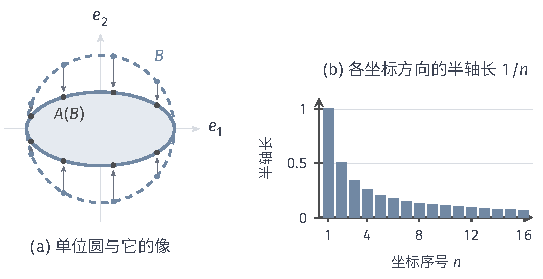
\includegraphics[width=91.9mm]{figures/02-abstract-mathematics/03-function-spaces/tikz/c3-compact-ellipse/figure.pdf}
  \caption{$\ell^2$上的$A(x_n)=(x_n/n)$怎样压缩单位球$B$。(a) 在$e_1,e_2$张成的平面上，虚线单位圆上的点沿箭头映到实线椭圆，椭圆半轴为$1$与$1/2$。(b) 像集$A(B)$的第$n$个坐标不超过$1/n$；越靠后的方向被压得越扁，这正是像集可以被有限个代表点近似覆盖的原因。}
  \label{fig:ose-compact-ellipse}
\end{figure}

\begin{definition}[紧算子]
\label{def:ose-compact-operator}
设$X,Y$为赋范空间，$A:X\to Y$为线性算子。若对$X$中每个有界序列$(x_n)$，输出序列$(Ax_n)$都有在$Y$中按范数收敛的子列，则称$A$为\term{紧算子}（compact operator）。等价地，单位球的像$A(B)$在$Y$中相对紧，即其闭包是紧集。
\end{definition}

紧算子必然有界：若$A$无界，可取单位向量$x_n$使$\|Ax_n\|\geq n$，输出序列的任何子列都无界，不可能收敛。由前面的讨论，每个有界有限秩算子都是紧算子。$A(x_n)=(x_n/n)$的紧性在第~\ref{sec:ose-finite-rank}小节用有限秩逼近给出简洁的证明。

\paragraph{单位算子不紧}
紧性不是每个有界算子都具备的。设$H$为无限维Hilbert空间，取标准正交序列$(e_n)$。对$n\neq m$，由正交性，
\[
  \|e_n-e_m\|^2=\|e_n\|^2+\|e_m\|^2=2 .
\]
单位算子$I$把这个有界序列原样输出，任意两项相距$\sqrt2$，任何子列都不是柯西列，因而没有收敛子列，$I$不是紧算子。同样的序列经过$A(x_n)=(x_n/n)$后变成$Ae_n=e_n/n$，它按范数趋于零。图~\ref{fig:ose-identity-orthonormal}对比了两种输出：左图中三个正交方向两两相距$\sqrt2$，而它们在$A$下的像向原点收拢；右图显示相邻输出的距离在单位算子下恒为$\sqrt2$，在$A$下逐渐趋于零。

\begin{figure}[!htb]
  \centering
  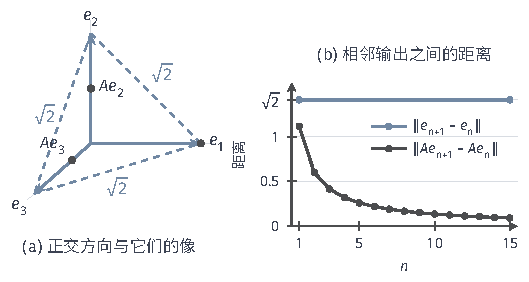
\includegraphics[width=89.6mm]{figures/02-abstract-mathematics/03-function-spaces/tikz/c3-identity-orthonormal/figure.pdf}
  \caption{同一个标准正交序列经过单位算子与经过$A(x_n)=(x_n/n)$的对比。(a) $e_1,e_2,e_3$两两相距$\sqrt2$（虚线），它们在$A$下的像$Ae_1=e_1$、$Ae_2=e_2/2$、$Ae_3=e_3/3$（黑点）向原点收拢。(b) 相邻输出的距离：单位算子下恒为$\sqrt2$，在$A$下等于$\sqrt{1/n^2+1/(n+1)^2}$并趋于零。}
  \label{fig:ose-identity-orthonormal}
\end{figure}

这个例子还提醒我们紧性约束的是什么。由第~\ref{sec:fs-orthogonal-expansion}节，每个$x\in H$都能被它在前$n$个基向量上的截断任意逼近；单独看每个函数，“有限截断”都可行。紧性要求的却是：同一个算子作用于整个有界输入族之后，输出整体可以被有限个代表覆盖。单位算子对每个输入都能截断，对整个单位球却不能，二者的差别正是逐个逼近与统一逼近的差别。

\paragraph{紧算子把弱收敛改善为范数收敛}
第~\ref{sec:lfo-weak-convergence}节已经看到，标准正交序列$e_n\rightharpoonup0$却不按范数收敛。上面的例子中，$Ae_n=e_n/n$按范数收敛到$A0=0$；这不是巧合，紧算子总能把弱收敛的输入变成按范数收敛的输出。

\begin{theorem}[紧算子改善收敛]
\label{thm:ose-compact-weak-strong}
设$X,Y$为赋范空间，$A:X\to Y$为紧算子。若$x_n\rightharpoonup x$，则$\|Ax_n-Ax\|\to0$。
\end{theorem}

\begin{proof}
第一步，说明输入有界、输出弱收敛。由第~\ref{sec:lfo-weak-norm}节，弱收敛序列有界，设$\sup_n\|x_n\|=C<\infty$。对每个$\ell\in Y^*$，复合$\ell\circ A$是$X$上的有界线性泛函，所以$\ell(Ax_n)=(\ell\circ A)(x_n)\to(\ell\circ A)(x)=\ell(Ax)$，即$Ax_n\rightharpoonup Ax$。这一步只用到$A$有界。

第二步，用反证法加上紧性。假设$Ax_n$不按范数收敛到$Ax$，则存在$\varepsilon>0$及子列$(x_{n_k})$，使$\|Ax_{n_k}-Ax\|\geq\varepsilon$对所有$k$成立。子列$(x_{n_k})$仍有界，由紧性可再抽出子列，使相应输出按范数收敛到某个$y\in Y$。

第三步，确认这个极限只能是$Ax$。范数收敛蕴含弱收敛，所以沿这个更细的子列，输出同时弱收敛到$y$和$Ax$。由第~\ref{sec:lfo-hahn-banach}节，连续线性泛函可以区分$Y$中不同的点，故弱极限唯一，$y=Ax$。这与$\|Ax_{n_k}-Ax\|\geq\varepsilon$矛盾。
\end{proof}

证明的分工很清楚：有界性只给出弱收敛被保持，紧性提供范数收敛的子列，弱极限的唯一性再把所有子列的极限钉在同一点。对一般有界算子，第二步不成立：单位算子把$e_n\rightharpoonup0$原样输出，输出仍只是弱收敛。

\subsection{有限秩逼近与算子范数}
\label{sec:ose-finite-rank}

上一小节的例子暗示，紧算子可以看作“有限秩算子的极限”。本小节把这一直觉分成两个方向：先证明紧算子的算子范数极限仍是紧算子，这给出构造紧算子的方法；再在Hilbert空间中证明反方向，即每个紧算子都能由有限秩算子按算子范数逼近。

\paragraph{算子范数极限保持紧性}
证明要用到第~\ref{sec:metric-complete-totally-bounded}节的定理~\ref{thm:metric-compact-complete-tb}：度量空间紧致当且仅当它完备且全有界，全有界指对每个$\varepsilon>0$都能被有限个半径$\varepsilon$的球覆盖。在完备空间$Y$中，全有界集合的闭包仍全有界，又作为闭子集完备，因而是紧集；所以要证像集相对紧，只需证它全有界。

\begin{theorem}[紧算子集合在算子范数下闭]
\label{thm:ose-compact-limit}
设$X$为赋范空间，$Y$为Banach空间，$A_n:X\to Y$都是紧算子，$A\in\mathcal B(X,Y)$且$\|A_n-A\|\to0$，则$A$是紧算子。
\end{theorem}

\begin{proof}
只需证明单位球的像$A(B)$全有界，再用$Y$的完备性得到闭包紧。给定$\varepsilon>0$，先取$n$使$\|A_n-A\|<\varepsilon$。由于$A_n$紧，$A_n(B)$全有界，存在有限个点$y_1,\ldots,y_N\in Y$，使每个$A_nx$（$x\in B$）都满足$\min_i\|A_nx-y_i\|<\varepsilon$。

对任意$x\in B$，选出相应的$y_i$，用三角不等式把误差拆成两段：
\[
  \|Ax-y_i\|\leq\|(A-A_n)x\|+\|A_nx-y_i\|<\|A-A_n\|\,\|x\|+\varepsilon<2\varepsilon .
\]
因此同一组$y_1,\ldots,y_N$是$A(B)$的有限$2\varepsilon$网。$\varepsilon$任意，$A(B)$全有界；$Y$完备，故$\overline{A(B)}$紧，$A$是紧算子。
\end{proof}

关键在于误差界$\|A-A_n\|$对单位球中的所有输入一致成立，于是$A_n$的有限覆盖可以整体搬给$A$。若只知道$A_nx\to Ax$对每个$x$成立，就无法这样搬运；第~\ref{sec:lfo-operator-convergence}节中投影$P_n\to I$逐点成立，而极限$I$恰好不紧。

\begin{example}[对角算子的有限秩逼近]
\label{ex:ose-diagonal-finite-rank}
在$\ell^2$上令$A(x_n)=(x_n/n)$，并令$A_m$只保留前$m$个坐标：$A_mx=(x_1,x_2/2,\ldots,x_m/m,0,0,\ldots)$。$A_m$的像落在前$m$个坐标张成的空间中，是有限秩算子。差$(A-A_m)x$只剩第$m+1$个坐标以后的部分，
\[
  \|(A-A_m)x\|^2=\sum_{n>m}\frac{|x_n|^2}{n^2}\leq\frac{1}{(m+1)^2}\sum_{n>m}|x_n|^2\leq\frac{\|x\|^2}{(m+1)^2},
\]
取$x=e_{m+1}$时等号成立，所以$\|A-A_m\|=1/(m+1)\to0$。由定理~\ref{thm:ose-compact-limit}，$A$是紧算子。
\end{example}

图~\ref{fig:ose-finite-rank-error}把这个误差与单位算子的截断作比较。若用坐标投影$P_m$去逼近单位算子，取$x=e_{m+1}$可知$\|I-P_m\|=1$，无论保留多少坐标，统一误差都不下降；对固定的$x$，误差$\|(I-P_m)x\|$却趋于零，只是趋于零的速度依赖$x$本身。对角算子$A$的截断误差则按$1/(m+1)$对所有单位输入同时下降。

\begin{figure}[!htb]
  \centering
  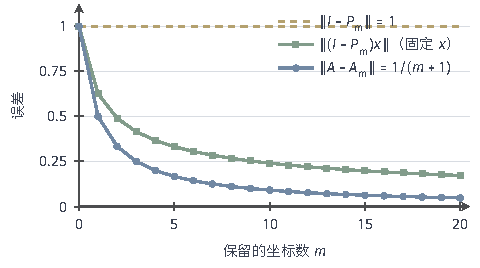
\includegraphics[width=81.2mm]{figures/02-abstract-mathematics/03-function-spaces/tikz/c3-finite-rank-error/figure.pdf}
  \caption{$\ell^2$上三种截断误差随保留坐标数$m$的变化。虚线：单位算子的统一误差$\|I-P_m\|$恒为$1$。方点：固定单位向量$x\propto(1/n)$的误差$\|(I-P_m)x\|$趋于零，但这一速度只属于这个$x$。圆点：紧算子$A(x_n)=(x_n/n)$的统一误差$\|A-A_m\|=1/(m+1)$。}
  \label{fig:ose-finite-rank-error}
\end{figure}

\paragraph{Hilbert空间中紧算子的有限秩逼近}
现在证明反方向。思路是：紧算子的像集可以被有限个点覆盖，这些点张成一个有限维子空间；向这个子空间作正交投影，就得到一个有限秩近似。正交投影的最近点性质（第~\ref{sec:fs-projection}节）保证投影误差不超过到覆盖点的距离。

\begin{theorem}[紧算子的有限秩逼近]
\label{thm:ose-finite-rank-approx}
设$X$为赋范空间，$H$为Hilbert空间，$A:X\to H$为紧算子。则存在有限秩算子$A_n:X\to H$，使$\|A-A_n\|\to0$。
\end{theorem}

\begin{proof}
给定$\varepsilon>0$。由紧性，$A(B)$全有界，取有限个点$y_1,\ldots,y_N$构成$A(B)$的$\varepsilon$网。令$M=\operatorname{span}\{y_1,\ldots,y_N\}$，它是有限维子空间，因而闭；设$P$为到$M$的正交投影，并令$F=PA$。$F$的像含于$M$，且$\|F\|\leq\|P\|\|A\|=\|A\|$，所以$F$是有界有限秩算子。

对任意$x\in B$，选$y_i$使$\|Ax-y_i\|<\varepsilon$。由于$PAx$是$M$中离$Ax$最近的点，而$y_i\in M$，
\[
  \|Ax-Fx\|=\|Ax-PAx\|\leq\|Ax-y_i\|<\varepsilon .
\]
对$x\in B$取上确界得$\|A-F\|\leq\varepsilon$。令$\varepsilon=1/n$，即得所需的有限秩算子列。
\end{proof}

证明中真正用到的是Hilbert空间的正交投影：它把有限覆盖转化为一个有界线性的“取最近点”操作。在一般Banach空间中，有限维子空间上不一定存在范数可控的投影，紧算子能否由有限秩算子按算子范数逼近，取决于空间是否具有所谓的逼近性质；确实存在不具有这一性质的Banach空间，所以本定理不能无条件推广。结合定理~\ref{thm:ose-compact-limit}，在Hilbert空间之间，紧算子恰好是有限秩算子的算子范数极限。后面的积分核逼近（第~\ref{sec:ose-hilbert-schmidt}节）和Fredholm二择的证明（第~\ref{sec:ose-fredholm}节）都会用到这一刻画。

% 第3章第2节：谱与奇异值（谱与特征值、紧自伴算子的谱分解、紧算子的奇异值分解）。

\section{谱与奇异值}
\label{sec:ose-spectrum}

紧算子能被有限秩算子统一逼近，但上一节没有说明应该保留哪些方向、每个方向被放大或压缩多少。有限维中，这个问题由特征值和奇异值回答。本节先用可逆性定义无限维算子的谱，说明它为什么不能只由特征值组成；再在紧自伴条件下建立正交的特征展开；最后对一般紧算子使用输入、输出两组方向，得到奇异值分解及最佳有限秩逼近。

\subsection{谱与特征值}
\label{sec:ose-spectrum-def}

\paragraph{从不可逆性定义谱}
在$n$维空间中，$\bm A-\lambda\bm I$不可逆当且仅当它不是单射，即存在非零向量$\bm v$使$\bm A\bm v=\lambda\bm v$；单射、满射和可逆三者等价，所以“使$\bm A-\lambda\bm I$不可逆的$\lambda$”恰好就是特征值。矩阵的特征值、实对称矩阵的正交对角化与奇异值分解都建立在这一等价关系上，可参考\BookChapterRef{chap:matrix-analysis}{卷一“谱和奇异值”章}。无限维中三者不再等价，必须直接从可逆性出发。

\begin{definition}[谱与预解集]
\label{def:ose-spectrum}
设$H$为复Hilbert空间，$A\in\mathcal B(H)$。若$A-\lambda I$是$H$到$H$的双射，且逆映射$(A-\lambda I)^{-1}$有界，则称$\lambda\in\mathbb C$属于$A$的\term{预解集}（resolvent set），记为$\rho(A)$，并称$(A-\lambda I)^{-1}$为\term{预解算子}（resolvent operator）。预解集的补集$\sigma(A)=\mathbb C\setminus\rho(A)$称为$A$的\term{谱}（spectrum）。若存在非零$u\in H$使$Au=\lambda u$，则称$\lambda$为$A$的\term{特征值}（eigenvalue），$u$为相应的\term{特征向量}（eigenvector）；在函数空间中也常称特征函数。
\end{definition}

由第~\ref{sec:lfo-open-mapping}节的有界逆定理，Banach空间之间的有界线性双射自动有有界逆，所以定义中“逆有界”一项对$A-\lambda I$是全空间双射的情形并不额外增加限制。写出这一项是为了强调：预解参数要求在\emph{整个}$H$上能够稳定地反解$(A-\lambda I)u=g$。特征值使$A-\lambda I$有非零核，当然属于谱；但$A-\lambda I$也可能是单射却不满射，此时只能在像上定义逆映射，这个逆映射还可能没有统一的界。这两种情形都使$\lambda$进入谱，却都不对应非零特征向量。

\paragraph{对角算子的谱}
回到$\ell^2$上的$A(x_n)=(x_n/n)$，逐个检查$\lambda$。若$\lambda=1/k$，则$Ae_k=e_k/k$，所以每个$1/k$都是特征值，特征向量为$e_k$。

再看$\lambda=0$。若$Ax=0$，则每个$x_n/n=0$，所以$A$是单射，$0$不是特征值。但$A$不是满射：第~\ref{sec:lfo-range-kernel}节已经说明，$y=(1/n)\in\ell^2$的唯一形式逆像是常数列$(1,1,\ldots)$，它不平方可和，故$y\notin\operatorname{Ran}A$。即使只在像上考虑逆映射$y\mapsto(ny_n)$，它把单位向量$e_n$送到$ne_n$，范数为$n$，没有统一的界。所以$0\in\sigma(A)$，却不是特征值。

最后取$\lambda$不在集合$S=\{1/n:n\geq1\}\cup\{0\}$中。$S$是闭集（它唯一的聚点$0$已在其中），所以$d=\operatorname{dist}(\lambda,S)>0$。对每个$n$有$|1/n-\lambda|\geq d$，于是方程$(A-\lambda I)x=y$逐坐标解出
\[
  x_n=\frac{y_n}{1/n-\lambda},\qquad \|x\|\leq\frac{1}{d}\|y\| .
\]
这给出全空间上的有界逆，$\lambda\in\rho(A)$。综合三种情形，
\[
  \sigma(A)=\{1/n:n\geq1\}\cup\{0\},\qquad \|(A-\lambda I)^{-1}\|=\frac{1}{\operatorname{dist}(\lambda,\sigma(A))}\quad(\lambda\in\rho(A)).
\]
范数公式中的上界刚刚得到；取$y=e_n$并让$1/n$逼近离$\lambda$最近的谱点，可知上界不能改进。

\begin{figure}[!htb]
  \centering
  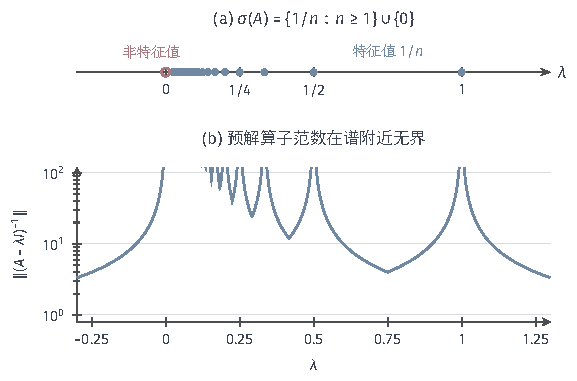
\includegraphics[width=97.8mm]{figures/02-abstract-mathematics/03-function-spaces/tikz/c3-spectrum-resolvent/figure.pdf}
  \caption{$\ell^2$上$A(x_n)=(x_n/n)$的谱。(a) 特征值$1/n$（实心点）向$0$聚集；$0$在谱中但不是特征值（空心点）。(b) 实参数$\lambda$处预解算子的范数$1/\operatorname{dist}(\lambda,\sigma(A))$，纵轴取对数；每个谱点附近范数都无界，在$0$附近这些尖峰挤在一起。}
  \label{fig:ose-spectrum-resolvent}
\end{figure}

图~\ref{fig:ose-spectrum-resolvent}把这三种情形放在一起：特征值是孤立的点，它们聚集到不是特征值的$0$；在任何谱点附近，反解$(A-\lambda I)u=g$的放大倍数都没有上界。三种情形对应三种不同的方向信息：特征值$1/n$对应被精确缩放的方向$e_n$；$0$不对应任何被消去的方向，而是对应一列被压得越来越扁的方向，使像空间稠密却不闭合；远离谱的$\lambda$则让每个方向的缩放倍数$1/n-\lambda$都离零有一段距离。

这一现象对紧算子是普遍的。若$H$无限维而紧算子$A$有有界逆，则$I=A^{-1}A$作为有界算子与紧算子的复合仍是紧算子（有界输入列经$A$后有收敛子列，再经连续的$A^{-1}$仍收敛），与第~\ref{sec:ose-compact-def}小节中单位算子不紧矛盾。所以无限维空间中的紧算子总有$0\in\sigma(A)$，无论$0$是否为特征值。

实Hilbert空间中的算子可以先扩张到复化空间再讨论谱；对下面的自伴算子，特征值都是实数，这样做不会产生新的困难。一般非自伴算子的谱可能含有非实数，其谱分类不在本章展开。

\subsection{紧自伴算子的谱分解}
\label{sec:ose-spectral-theorem}

对角算子的例子中，特征向量$e_n$恰好组成标准正交基，算子就是沿每个基方向乘以一个数。实对称矩阵具有同样的结构：存在由特征向量组成的标准正交基，矩阵在这组基下是实对角矩阵。本小节证明，紧自伴算子在无限维中保留了这一结构：非零特征值至多可数并只能聚集到零，特征方向两两正交，并且与核一起张满整个空间。

\paragraph{紧自伴谱分解的陈述}
自伴算子的定义见第~\ref{sec:lfo-self-adjoint}节：$A\in\mathcal B(H)$满足$A^*=A$，即$\langle v,Au\rangle=\langle Av,u\rangle$对所有$u,v$成立。

\begin{theorem}[紧自伴算子的谱分解]
\label{thm:ose-compact-selfadjoint}
设$H$为实或复Hilbert空间，$A:H\to H$为紧自伴算子。则：
\begin{enumerate}
  \item $A$的特征值都是实数，属于不同特征值的特征向量互相正交；
  \item 每个非零特征值的特征空间有限维；对每个$\delta>0$，满足$|\lambda|\geq\delta$的特征值只有有限个，因此非零特征值至多可数，并且只可能在$0$处聚集；
  \item 存在有限或可数的标准正交序列$(e_j)$及非零实数$\lambda_j$（按重数重复列出，$|\lambda_1|\geq|\lambda_2|\geq\cdots$，序列无限时$\lambda_j\to0$），使$Ae_j=\lambda_je_j$，$(e_j)$的闭张成等于$(\ker A)^\perp$，并且对每个$u\in H$，
  \begin{equation}
    u=u_0+\sum_j\langle e_j,u\rangle e_j,\qquad Au=\sum_j\lambda_j\langle e_j,u\rangle e_j,\qquad u_0\in\ker A,
    \label{eq:ose-spectral-expansion}
  \end{equation}
  两个级数都按$H$的范数收敛。
\end{enumerate}
\end{theorem}

证明的主线是：先说明自伴算子的范数可以由二次型$\langle u,Au\rangle$读出，再用紧性找到使二次型绝对值达到最大的方向，它就是一个特征方向；然后把算子限制到这个方向的正交补上，重复同样的步骤。下面分步完成。

\paragraph{特征值与正交性}
设$Au=\lambda u$，$u\neq0$。由内积对第二变量线性、对第一变量共轭线性，$\langle u,Au\rangle=\lambda\|u\|^2$，$\langle Au,u\rangle=\overline\lambda\|u\|^2$；自伴使两者相等，所以$\lambda=\overline\lambda$为实数。再设$Av=\mu v$，$\mu\neq\lambda$，两者都是实数，于是
\[
  \lambda\langle v,u\rangle=\langle v,Au\rangle=\langle Av,u\rangle=\mu\langle v,u\rangle ,
\]
从而$\langle v,u\rangle=0$。这证明了结论1。

\paragraph{非零特征值的有限性}
设$(e_j)$是一列两两正交的单位特征向量，$Ae_j=\lambda_je_j$且$|\lambda_j|\geq\delta>0$。这种序列可以来自同一个特征空间的标准正交组，也可以来自不同特征值（由结论1自动正交）。对$j\neq k$，
\[
  \|Ae_j-Ae_k\|^2=\|\lambda_je_j-\lambda_ke_k\|^2=|\lambda_j|^2+|\lambda_k|^2\geq2\delta^2 ,
\]
输出列没有柯西子列，与紧性矛盾。所以这种序列只能有限长。取同一特征空间中的标准正交组，即知非零特征空间有限维；取不同特征值的特征向量，即知$|\lambda|\geq\delta$的特征值只有有限个。令$\delta=1,1/2,1/3,\ldots$，非零特征值是可数个有限集合的并，且任何$\delta>0$之外只有有限个，只能在$0$处聚集。这证明了结论2。

\paragraph{二次型给出范数}
设$A$自伴，令$M=\sup_{\|u\|=1}|\langle u,Au\rangle|$。由Cauchy–Schwarz不等式，$|\langle u,Au\rangle|\leq\|A\|$，故$M\leq\|A\|$。反向不等式要从二次型恢复$\|Au\|$。自伴性使$\langle u,Au\rangle=\langle Au,u\rangle=\overline{\langle u,Au\rangle}$为实数，展开可得
\[
  \langle u+v,A(u+v)\rangle-\langle u-v,A(u-v)\rangle=2\langle u,Av\rangle+2\langle v,Au\rangle=4\operatorname{Re}\langle v,Au\rangle ,
\]
其中用到$\langle u,Av\rangle=\langle Au,v\rangle=\overline{\langle v,Au\rangle}$。左边两项各自的绝对值不超过$M\|u\pm v\|^2$，再用平行四边形恒等式$\|u+v\|^2+\|u-v\|^2=2\|u\|^2+2\|v\|^2$，
\[
  4\operatorname{Re}\langle v,Au\rangle\leq M\bigl(\|u+v\|^2+\|u-v\|^2\bigr)=2M\bigl(\|u\|^2+\|v\|^2\bigr).
\]
对单位向量$u$且$Au\neq0$，取$v=Au/\|Au\|$，则$\operatorname{Re}\langle v,Au\rangle=\|Au\|$，上式化为$4\|Au\|\leq4M$。因此$\|A\|\leq M$，两者相等。

\paragraph{紧性给出极值方向}
现设$A\neq0$紧自伴。取单位向量$u_n$使$|\langle u_n,Au_n\rangle|\to\|A\|$。这些二次型都是实数，绝对值趋于$\|A\|>0$，可以抽出子列使它们的符号一致，于是沿该子列$\langle u_n,Au_n\rangle\to\lambda$，其中$\lambda=\|A\|$或$\lambda=-\|A\|$。这里不能预先假定$\lambda$为正：自伴算子的二次型可以取负值，绝对值最大的特征值可能是负的。展开
\[
  \|Au_n-\lambda u_n\|^2=\|Au_n\|^2-2\lambda\langle u_n,Au_n\rangle+\lambda^2\leq2\lambda^2-2\lambda\langle u_n,Au_n\rangle\to0 ,
\]
其中用到$\|Au_n\|\leq\|A\|=|\lambda|$。由紧性，可再抽子列使$Au_n\to w$。于是$\lambda u_n=Au_n-(Au_n-\lambda u_n)\to w$，即$u_n\to e=w/\lambda$，且$\|e\|=1$。由$A$连续，$Ae=\lim Au_n=w=\lambda e$。所以$\pm\|A\|$中至少有一个是特征值，且对应单位特征向量$e$。

\paragraph{逐步分解与核}
记$e_1=e$，$\lambda_1=\lambda$。正交补$H_2=\{e_1\}^\perp$在$A$下不变：若$\langle e_1,v\rangle=0$，则$\langle e_1,Av\rangle=\langle Ae_1,v\rangle=\lambda_1\langle e_1,v\rangle=0$。$A$在$H_2$上的限制仍是紧自伴算子，范数不超过$\|A\|$。若这个限制为零，过程停止；否则对它重复上一段，得到$e_2\perp e_1$及$|\lambda_2|=\|A|_{H_2}\|\leq|\lambda_1|$。依此类推，在$H_k=\{e_1,\ldots,e_{k-1}\}^\perp$上取$e_k$，得到$|\lambda_1|\geq|\lambda_2|\geq\cdots$。若过程不停止，由结论2，$\lambda_k\to0$。

令$M$为$(e_j)$的闭张成。$M^\perp$含于每个$H_k$，所以$A$在$M^\perp$上的限制的范数不超过每个$|\lambda_k|$；过程无限时它趋于零，有限时按停止条件本身为零。因此$A$在$M^\perp$上恒为零，$M^\perp\subseteq\ker A$。反过来，若$Au=0$，则对每个$j$，
\[
  \langle e_j,u\rangle=\frac{1}{\lambda_j}\langle Ae_j,u\rangle=\frac{1}{\lambda_j}\langle e_j,Au\rangle=0 ,
\]
所以$\ker A\subseteq M^\perp$。二者相等，$M=(M^\perp)^\perp=(\ker A)^\perp$。这同时说明每个非零特征值都已出现在$(\lambda_j)$中：属于非零特征值$\mu$的特征向量与$\ker A$正交，因而落在$M$中；若$\mu$不等于任何$\lambda_j$，它就与所有$e_j$正交，只能为零。

\paragraph{展开式}
由第~\ref{sec:fs-orthogonal-expansion}节，$u$在闭子空间$M$上的正交投影为$\sum_j\langle e_j,u\rangle e_j$，级数按范数收敛；余项$u_0$属于$M^\perp=\ker A$。把$A$作用于投影的部分和，由连续性得到$Au=\sum_j\lambda_j\langle e_j,u\rangle e_j$。这就是式~\eqref{eq:ose-spectral-expansion}，证毕。

\paragraph{贯穿例子中的谱分解}
在$L^2([-1,1],\mu)$上，$d\mu=dz/2$，核$K(x,z)=1+xz$给出$(Tf)(x)=\int f\,d\mu+x\int zf\,d\mu$。由$\int1\,d\mu=1$与$\int z^2\,d\mu=\frac12\int_{-1}^{1}z^2\,dz=\frac13$，
\[
  T1=1,\qquad Tx=x\int z^2\,d\mu=\tfrac13x .
\]
单位化得$e_1=1$、$e_2=\sqrt3\,x$（因为$\int3x^2\,d\mu=1$），特征值$\lambda_1=1$、$\lambda_2=1/3$。式~\eqref{eq:ose-spectral-expansion}化为
\[
  Tf=\langle e_1,f\rangle e_1+\tfrac13\langle e_2,f\rangle e_2 ,
\]
与$1,x$都正交的函数组成$\ker T$，它是无限维的。第~\ref{sec:ose-kernels}小节将在积分核的语言下再看这个例子。

把核换成$1-6xz$，常数方向不变，线性方向变为$T x=-6x\int z^2\,d\mu=-2x$，特征值$-2$的绝对值最大。图~\ref{fig:ose-spectral-stretch}(b)在$e_1,e_2$的系数平面上画出单位圆的像：沿$e_1$方向不变，沿$e_2$方向拉长两倍并翻转，点$p$被送到$e_2$坐标反号的$Tp$。若只寻找正的最大特征值，就会漏掉这个主导方向。图~\ref{fig:ose-spectral-stretch}(a)则显示$\ell^2$对角算子的情形：$u$的每个系数$\langle e_j,u\rangle$被乘以$\lambda_j=1/j$，后面的方向被压得更小。

\begin{figure}[!htb]
  \centering
  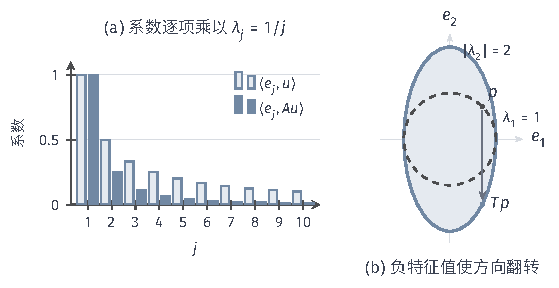
\includegraphics[width=94.6mm]{figures/02-abstract-mathematics/03-function-spaces/tikz/c3-spectral-stretch/figure.pdf}
  \caption{紧自伴算子沿特征方向逐个伸缩。(a) $\ell^2$上$A=\operatorname{diag}(1/j)$，浅色条为$u$的系数$\langle e_j,u\rangle=1/j$，深色条为$Au$的系数$1/j^2$。(b) $L^2([-1,1],dz/2)$上核$1-6xz$的积分算子，在$e_1=1$、$e_2=\sqrt3x$的系数平面上把虚线单位圆映为实线椭圆：$e_1$方向乘$1$，$e_2$方向乘$-2$。与$1,x$正交的方向全部被映为零，图中未画出。}
  \label{fig:ose-spectral-stretch}
\end{figure}

\paragraph{展开的收敛方式}
式~\eqref{eq:ose-spectral-expansion}中的级数按Hilbert空间的范数收敛。对$L^2(\mu)$中的函数，这意味着平方积分误差趋于零，并不意味着在每个点或一致地收敛；$L^2$的元素本来就是几乎处处等价类，单独谈某一点的值没有意义。若要把特征展开写成核函数$K(x,z)=\sum_j\lambda_je_j(x)\overline{e_j(z)}$的逐点甚至一致收敛的级数，需要核连续、半正定等额外条件，这是第~\ref{sec:rkhs-mercer}节Mercer定理讨论的内容。

\subsection{紧算子的奇异值分解}
\label{sec:ose-svd}

非自伴算子不一定有足够多的特征向量，输入与输出甚至可以位于不同的空间。有限维中，矩阵的奇异值分解用输入、输出各一组标准正交方向解决这个问题。对紧算子，同样的构造可以通过正紧自伴算子$A^*A$完成。

\paragraph{从$A^*A$构造两组方向}
设$H_1,H_2$为Hilbert空间，$A:H_1\to H_2$为紧算子。$A^*A:H_1\to H_1$是紧算子：有界输入列经$A$后有收敛子列，再经连续的$A^*$仍收敛。它也是自伴的，且
\[
  \langle x,A^*Ax\rangle=\langle Ax,Ax\rangle=\|Ax\|^2\geq0 ,
\]
所以它的特征值都非负，并且$A^*Ax=0$当且仅当$Ax=0$，即$\ker(A^*A)=\ker A$。

对$A^*A$应用定理~\ref{thm:ose-compact-selfadjoint}，得到标准正交的特征向量$v_j$与正特征值$s_j$，按递减顺序排列。令$\sigma_j=\sqrt{s_j}$，再令$u_j=Av_j/\sigma_j$。这组输出方向也是标准正交的：
\[
  \langle u_j,u_k\rangle=\frac{\langle Av_j,Av_k\rangle}{\sigma_j\sigma_k}=\frac{\langle v_j,A^*Av_k\rangle}{\sigma_j\sigma_k}=\frac{\sigma_k^2\langle v_j,v_k\rangle}{\sigma_j\sigma_k}=\delta_{j,k} .
\]
此外$A^*u_j=A^*Av_j/\sigma_j=\sigma_jv_j$，所以$A$把$v_j$送到$\sigma_ju_j$，$A^*$把$u_j$送回$\sigma_jv_j$。

\begin{theorem}[紧算子的奇异值分解]
\label{thm:ose-svd}
设$A:H_1\to H_2$为紧算子，$\sigma_1\geq\sigma_2\geq\cdots>0$及标准正交序列$(v_j)\subset H_1$、$(u_j)\subset H_2$如上构造。则对每个$x\in H_1$、$y\in H_2$，
\begin{equation}
  Ax=\sum_j\sigma_j\langle v_j,x\rangle u_j,\qquad A^*y=\sum_j\sigma_j\langle u_j,y\rangle v_j ,
  \label{eq:ose-svd}
\end{equation}
级数按范数收敛。$(v_j)$的闭张成为$(\ker A)^\perp$，$(u_j)$的闭张成为$\overline{\operatorname{Ran}A}=(\ker A^*)^\perp$。序列无限时$\sigma_j\to0$。
\end{theorem}

\begin{proof}
由定理~\ref{thm:ose-compact-selfadjoint}，$(v_j)$的闭张成为$(\ker A^*A)^\perp=(\ker A)^\perp$，任意$x$可写成$x=x_0+\sum_j\langle v_j,x\rangle v_j$，$x_0\in\ker A$。把$A$作用于部分和并取极限，得$Ax=\sum_j\langle v_j,x\rangle Av_j=\sum_j\sigma_j\langle v_j,x\rangle u_j$。由这一展开，每个$Ax$都落在$(u_j)$的闭张成中；反之每个$u_j=A(v_j/\sigma_j)$属于$\operatorname{Ran}A$。所以$(u_j)$的闭张成等于$\overline{\operatorname{Ran}A}$，再由第~\ref{sec:lfo-range-kernel}节得它等于$(\ker A^*)^\perp$。关于$A^*$的展开，对任意$x$有
\[
  \langle x,A^*y\rangle=\langle Ax,y\rangle=\sum_j\sigma_j\overline{\langle v_j,x\rangle}\langle u_j,y\rangle=\Bigl\langle x,\sum_j\sigma_j\langle u_j,y\rangle v_j\Bigr\rangle ,
\]
右端级数因系数平方可和而收敛，两边对所有$x$相等，故展开成立。$\sigma_j\to0$来自$s_j\to0$。
\end{proof}

数$\sigma_j$称为$A$的\term{奇异值}（singular value），$v_j$与$u_j$分别称为\term{右奇异向量}（right singular vector）与\term{左奇异向量}（left singular vector）。展开式~\eqref{eq:ose-svd}说明$A$的作用分三步：读出输入在$v_j$方向上的系数，乘以$\sigma_j$，再放到输出方向$u_j$上。输入中的$\ker A$完全看不见；输出中的$\ker A^*$则是永远到达不了的方向。两组方向一般属于不同的空间，即使$H_1=H_2$，$u_j$也未必等于$v_j$；只有正自伴算子才使两组方向重合、奇异值等于特征值。

\begin{example}[积分算子的奇异值分解]
\label{ex:ose-volterra-svd}
在$L^2(0,1)$上（Lebesgue测度），令$(Vf)(x)=\int_0^xf(t)\,dt$。它是核$\mathbf 1_{\{t<x\}}$的积分算子；这个核在$[0,1]^2$上平方可积，第~\ref{sec:ose-hilbert-schmidt}小节将证明这样的积分算子是紧算子，这里先承认这一点。由Fubini定理交换积分次序，伴随为$(V^*g)(t)=\int_t^1g(x)\,dx$，于是
\[
  (V^*Vf)(t)=\int_t^1\Bigl(\int_0^xf(s)\,ds\Bigr)dx .
\]

设$V^*Vf=sf$，$s>0$。右端是连续函数，所以$f=s^{-1}V^*Vf$连续；于是$Vf$连续可微，$V^*Vf$二次连续可微，$f$也二次连续可微。对$t$求导两次得$(V^*Vf)'=-Vf$、$(V^*Vf)''=-f$，因此$sf''=-f$；又由表达式直接读出$(V^*Vf)'(0)=0$、$(V^*Vf)(1)=0$，故$f'(0)=0$、$f(1)=0$。满足这些条件的非零解为$f(t)=c\cos(\omega t)$，其中$\omega=s^{-1/2}$且$\cos\omega=0$，即$\omega_k=(k-\tfrac12)\pi$，$k=1,2,\ldots$。

$V$是单射：若$\int_0^xf=0$对所有$x$成立，则$E\mapsto\int_Ef^+$与$E\mapsto\int_Ef^-$在所有区间上相等，由定理~\ref{thm:measure-pi-lambda-uniqueness}在全部Borel集上相等，取$E=\{f>0\}$即知$f\leq0$几乎处处，同理$f\geq0$几乎处处。于是$\ker V^*V=\ker V=\{0\}$，由定理~\ref{thm:ose-compact-selfadjoint}，$V^*V$的特征向量张满整个$L^2(0,1)$。由此得到
\[
  \sigma_k=\frac{1}{(k-\frac12)\pi}=\frac{2}{(2k-1)\pi},\qquad
  \begin{aligned}
    v_k(t)&=\sqrt2\cos\bigl((k-\tfrac12)\pi t\bigr),\\
    u_k(x)&=\sqrt2\sin\bigl((k-\tfrac12)\pi x\bigr),
  \end{aligned}
\]
其中$u_k=Vv_k/\sigma_k$可直接积分验证。前几个奇异值约为$0.637$、$0.212$、$0.127$、$0.091$，按$1/k$的速度衰减。
\end{example}

\paragraph{截断奇异值与最佳有限秩逼近}
奇异值分解直接给出有限秩逼近：只保留前$m$项，
\[
  A_mx=\sum_{j\leq m}\sigma_j\langle v_j,x\rangle u_j .
\]
下面的定理说明这个截断的误差恰为下一个奇异值，并且没有任何秩不超过$m$的算子做得更好。若正奇异值只有有限个，约定用尽之后的$\sigma_j=0$。

\begin{theorem}[截断奇异值分解的最优性]
\label{thm:ose-svd-truncation}
在定理~\ref{thm:ose-svd}的条件下，$\|A-A_m\|=\sigma_{m+1}$；对每个秩不超过$m$的有界算子$F:H_1\to H_2$，都有$\|A-F\|\geq\sigma_{m+1}$。
\end{theorem}

\begin{proof}
第一步，计算截断误差。由式~\eqref{eq:ose-svd}及$(u_j)$的正交性，
\[
  \|(A-A_m)x\|^2=\sum_{j>m}\sigma_j^2|\langle v_j,x\rangle|^2\leq\sigma_{m+1}^2\sum_{j>m}|\langle v_j,x\rangle|^2\leq\sigma_{m+1}^2\|x\|^2 ,
\]
其中最后一步是Bessel不等式。取$x=v_{m+1}$时等号成立（若$\sigma_{m+1}=0$，结论已由上式得到），所以$\|A-A_m\|=\sigma_{m+1}$。

第二步，证明下界。不妨设$\sigma_{m+1}>0$。令$W=\operatorname{span}\{v_1,\ldots,v_{m+1}\}$，它是$m+1$维的。$F$在$W$上的限制把$W$映入维数不超过$m$的$\operatorname{Ran}F$，由线性代数的维数公式，存在单位向量$x\in W$使$Fx=0$。写$x=\sum_{j\leq m+1}c_jv_j$，$\sum_j|c_j|^2=1$，则
\[
  \|(A-F)x\|^2=\|Ax\|^2=\sum_{j\leq m+1}\sigma_j^2|c_j|^2\geq\sigma_{m+1}^2 .
\]
因此$\|A-F\|\geq\sigma_{m+1}$。
\end{proof}

\begin{figure}[!htb]
  \centering
  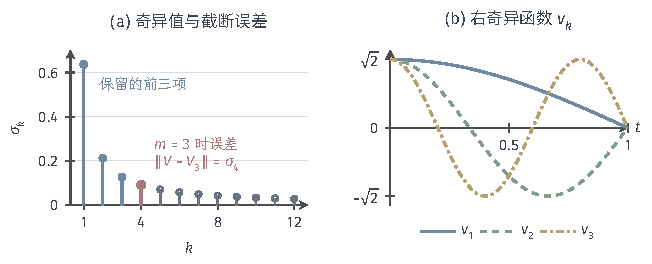
\includegraphics[width=110.3mm]{figures/02-abstract-mathematics/03-function-spaces/tikz/c3-svd-decay/figure.pdf}
  \caption{积分算子$(Vf)(x)=\int_0^xf$在$L^2(0,1)$上的奇异值分解。(a) 奇异值$\sigma_k=2/((2k-1)\pi)$；保留前三项（蓝色）时，算子范数误差等于第四个奇异值$\sigma_4\approx0.091$（红色），后面的奇异值（空心）全部被舍去。(b) 前三个右奇异函数$v_k(t)=\sqrt2\cos((k-\frac12)\pi t)$，序号越大振荡越快。}
  \label{fig:ose-svd-decay}
\end{figure}

图~\ref{fig:ose-svd-decay}在积分算子$V$上展示这一结论。保留前三项时误差为$\sigma_4\approx0.091$；奇异值衰减越快，同样秩的截断误差越小。右图显示，奇异值越小的方向振荡越快：$V$是积分，它把快速振荡的输入平均掉，输出的幅度只剩$1/\omega_k$倍。对比$\ell^2$上的$A(x_n)=(x_n/n)$，它是正自伴算子，奇异值就是特征值$1/n$，左右奇异向量都是$e_n$，例~\ref{ex:ose-diagonal-finite-rank}中的截断正是截断奇异值分解。

小奇异值对正向逼近是好消息：它们可以被舍去而误差很小。对反向求解却是坏消息：要从输出恢复输入，必须把这些方向上的系数除以$\sigma_j$。这一障碍留到第~\ref{sec:ose-first-kind}小节处理。

% 第3章第3节：积分算子（积分核与函数变换、平方可积核与紧性、核的对称性与算子伴随）。

\section{积分算子}
\label{sec:ose-integral-operators}

前两节的结论针对抽象的紧算子。本节用积分核具体地实现它们：先检查积分公式在什么意义下定义一个算子，再给出有界与紧所需的平方可积条件，最后把核的对称性与伴随、自伴联系起来。贯穿全节的一个提醒是：同一个核公式只有连同输入空间、输出空间和测度一起给出，才确定一个算子。

\subsection{积分核与函数变换}
\label{sec:ose-kernels}

\paragraph{积分公式的三个待查问题}
设$(X,\mu)$与$(Y,\nu)$为$\sigma$有限测度空间，$K:Y\times X\to\mathbb F$关于乘积$\sigma$代数可测。对$X$上的函数$f$，形式地定义
\begin{equation}
  (Tf)(y)=\int_XK(y,x)f(x)\,d\mu(x),\qquad y\in Y .
  \label{eq:ose-integral-operator}
\end{equation}
称$K$为\term{积分核}（integral kernel），$T$为以$K$为核的\term{积分算子}（integral operator）。核的第一个变量是输出位置，第二个变量是输入位置：固定$y$时，$K(y,\cdot)$是对输入$f$加权平均所用的权重。

公式~\eqref{eq:ose-integral-operator}本身只是一个形式表达。要让它确实定义一个算子$T:L^p(\mu)\to L^q(\nu)$，需要依次检查三件事：对哪些$y$，积分绝对收敛；把这些积分值拼成的函数$y\mapsto(Tf)(y)$是否可测；它是否属于目标空间$L^q(\nu)$。由于输入$f$只是几乎处处等价类，积分值不受$f$在零测集上改动的影响；输出也只能确定到$\nu$几乎处处，即$Tf$同样是一个等价类。第~\ref{sec:ose-hilbert-schmidt}小节将在平方可积的条件下完成这三项检查。

\paragraph{三种“核”的区别}
“核”这个词在本书中有几种不同的用法，不能因为名称相同就沿用相同的条件。第~\ref{sec:cond-kernels}节的概率核为每个输入点指定一个概率测度，要求非负且总质量为一，表示随机转移；第~\ref{sec:rkhs-kernel-properties}节的正定核要求对所有有限点集形成的Gram矩阵半正定，用来构造点值读取连续的函数空间。本节的积分核只是一个标量函数，可以取负值，不要求归一化，也不要求对称或正定；它通过积分把一个函数变成另一个函数。

\paragraph{贯穿例子：核如何选择方向}
在$X=Y=[-1,1]$上取$d\mu(z)=dz/2$与$K(x,z)=1+xz$。核可以拆成两个分离变量的乘积之和：$K(x,z)=1\cdot1+x\cdot z$。代入公式~\eqref{eq:ose-integral-operator}，
\[
  (Tf)(x)=\int_{-1}^{1}f\,d\mu+x\int_{-1}^{1}zf(z)\,d\mu(z) .
\]
输出总是一次函数，系数分别是输入的零阶矩与一阶矩。取$f=1+x$，由$\int(1+z)\,d\mu=1$与$\int z(1+z)\,d\mu=\int z^2\,d\mu=1/3$，得$Tf=1+x/3$：常数部分原样保留，斜率被压到原来的三分之一。再取$q(x)=x^2-1/3$，它的零阶矩$\int z^2\,d\mu-1/3=0$，一阶矩是奇函数的积分，也为零，所以$Tq=0$。

\begin{figure}[!htb]
  \centering
  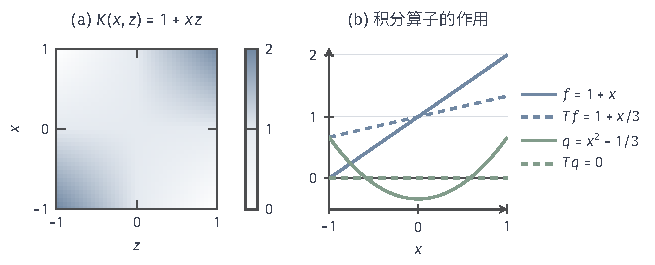
\includegraphics[width=110.9mm]{figures/02-abstract-mathematics/03-function-spaces/tikz/c3-kernel-action/figure.pdf}
  \caption{核$K(x,z)=1+xz$及其积分算子在$L^2([-1,1],dz/2)$上的作用。(a) 核的热图，颜色越深取值越大；沿对角方向$xz>0$时权重大于$1$。(b) $f=1+x$被映为$Tf=1+x/3$，常数方向保留、线性方向乘$1/3$；与$1,x$都正交的$q=x^2-1/3$被映为零。}
  \label{fig:ose-kernel-action}
\end{figure}

图~\ref{fig:ose-kernel-action}把核与作用放在一起。左图中的权重随$x,z$同号或异号而增减，正是这种结构使输出只记住输入的“平均”和“倾斜”；右图中，$q$虽然不是零函数，却与两个被记住的方向都正交，因而完全被消去。用第~\ref{sec:ose-spectral-theorem}小节的语言，$1$与$\sqrt3x$是特征值$1$与$1/3$的特征函数，$q$属于无限维的核空间。由于输出落在二维空间$\operatorname{span}\{1,x\}$中，$T$是秩为$2$的有限秩算子；一般地，$K(y,x)=\sum_{i=1}^r\varphi_i(y)\psi_i(x)$这类分离变量的有限和总给出秩不超过$r$的积分算子。

\paragraph{测度是算子的一部分}
保持核公式不变，把测度换成Lebesgue测度$dz$，两个矩都加倍，算子变成
\[
  (\tilde Tf)(x)=\int_{-1}^{1}(1+xz)f(z)\,dz=2\int f\,d\mu+2x\int zf\,d\mu ,
\]
于是$\tilde T(1+x)=2+2x/3$，特征值变为$2$与$2/3$，单位特征函数也随新内积重新归一化。同一个核在不同测度下给出不同的算子，谱也随之改变；讨论积分算子的谱时，必须同时报告核和测度。

\subsection{平方可积核与紧性}
\label{sec:ose-hilbert-schmidt}

现在给出一个容易检查的条件，使公式~\eqref{eq:ose-integral-operator}定义$L^2(\mu)$到$L^2(\nu)$的有界算子，并进一步是紧算子。下面用到的乘积测度与一般测度空间上的Tonelli、Fubini定理见本卷第~\ref{sec:integral-iterated}节（定理~\ref{thm:analysis-tonelli-fubini}与定理~\ref{thm:integral-fubini}）。

\paragraph{有界性}
逐点看，$(Tf)(y)$是截面$K(y,\cdot)$与$f$的内积，Cauchy–Schwarz不等式控制它的大小；再对$y$平方积分，截面范数的平方积分恰好是核的$L^2$范数平方。

\begin{theorem}[平方可积核的有界性]
\label{thm:ose-hs-bounded}
设$(X,\mu)$、$(Y,\nu)$为$\sigma$有限测度空间，$K\in L^2(\nu\otimes\mu)$。则对每个$f\in L^2(\mu)$，积分~\eqref{eq:ose-integral-operator}对$\nu$几乎每个$y$绝对收敛，$Tf\in L^2(\nu)$，且
\begin{equation}
  \|Tf\|_{L^2(\nu)}\leq\|K\|_{L^2(\nu\otimes\mu)}\|f\|_{L^2(\mu)},\qquad\text{从而}\quad\|T\|\leq\|K\|_{L^2(\nu\otimes\mu)} .
  \label{eq:ose-hs-bound}
\end{equation}
\end{theorem}

\begin{proof}
第一步，取得平方可积的截面。对非负函数$|K|^2$用Tonelli定理，
\[
  \int_Y\Bigl(\int_X|K(y,x)|^2\,d\mu(x)\Bigr)d\nu(y)=\|K\|_{L^2(\nu\otimes\mu)}^2<\infty ,
\]
所以内层积分对$\nu$几乎每个$y$有限，即截面$K(y,\cdot)\in L^2(\mu)$几乎处处成立。

第二步，逐点估计。对这样的$y$，由Cauchy–Schwarz不等式，
\[
  \int_X|K(y,x)f(x)|\,d\mu(x)\leq\|K(y,\cdot)\|_{L^2(\mu)}\|f\|_{L^2(\mu)}<\infty ,
\]
积分绝对收敛，且$|(Tf)(y)|\leq\|K(y,\cdot)\|_{L^2(\mu)}\|f\|_{L^2(\mu)}$。可测性也由Fubini定理得到：在任一有限测度的可测集$E\subseteq Y$上，对上式关于$y$积分并再用一次Cauchy–Schwarz不等式，
\[
  \int_E\int_X|K(y,x)f(x)|\,d\mu(x)\,d\nu(y)\leq\nu(E)^{1/2}\|K\|_{L^2(\nu\otimes\mu)}\|f\|_{L^2(\mu)}<\infty ,
\]
所以$(y,x)\mapsto K(y,x)f(x)$在$E\times X$上可积，内层积分$y\mapsto(Tf)(y)$在$E$上可测；$Y$是可数个这样的集合之并。

第三步，对$y$积分。把第二步的逐点界平方后积分，
\[
  \|Tf\|_{L^2(\nu)}^2\leq\int_Y\|K(y,\cdot)\|_{L^2(\mu)}^2\,d\nu(y)\,\|f\|_{L^2(\mu)}^2=\|K\|_{L^2(\nu\otimes\mu)}^2\|f\|_{L^2(\mu)}^2 .
\]
线性显然，于是$T$是有界线性算子，且式~\eqref{eq:ose-hs-bound}成立。
\end{proof}

平方可积核给出的积分算子称为\term{Hilbert--Schmidt积分算子}（Hilbert--Schmidt integral operator）。在贯穿例子中，
\[
  \|K\|_{L^2(\mu\otimes\mu)}^2=\iint(1+xz)^2\,d\mu(x)\,d\mu(z)=1+2\cdot0+\tfrac13\cdot\tfrac13=\tfrac{10}{9},
\]
而$\|T\|=1$（最大特征值），确实满足$\|T\|\leq\sqrt{10/9}$。注意$10/9=1^2+(1/3)^2$恰好是特征值的平方和；对例~\ref{ex:ose-volterra-svd}的积分算子$V$，$\|\mathbf 1_{\{t<x\}}\|_{L^2}^2=1/2$，而$\sum_k\sigma_k^2=\frac{4}{\pi^2}\sum_k\frac{1}{(2k-1)^2}=\frac{4}{\pi^2}\cdot\frac{\pi^2}{8}=\frac12$。可以证明，核的$L^2$范数平方总等于奇异值的平方和，这里只把它作为两个例子中的数值核对。

\paragraph{平方可积只是充分条件}
有界积分算子的核不必平方可积。取$X=Y=\mathbb N$，$\mu=\nu$为计数测度，此时$L^2$就是$\ell^2$，积分就是求和。核$K(m,n)=\mathbf 1_{\{m=n\}}$给出$(Tf)(m)=\sum_nK(m,n)f(n)=f(m)$，即单位算子，它有界而且范数为$1$；但$\|K\|_{L^2}^2=\sum_{m,n}K(m,n)^2$是无穷多个$1$之和，发散。由第~\ref{sec:ose-compact-def}小节，这个算子也不是紧算子。所以定理~\ref{thm:ose-hs-bounded}只说平方可积够用，不说有界算子都必须如此。

\paragraph{用矩形核逼近}
紧性的证明沿用第~\ref{sec:ose-finite-rank}小节的路线：把算子写成有限秩算子的算子范数极限。式~\eqref{eq:ose-hs-bound}说明核的$L^2$误差控制算子范数误差，所以只需用分离变量的有限和逼近核。最简单的分离变量核是矩形示性函数$\mathbf 1_{B\times A}(y,x)=\mathbf 1_B(y)\mathbf 1_A(x)$，下面的引理说明它们的线性组合足够用。

\begin{lemma}[矩形逼近]
\label{lem:ose-rectangle-approx}
设$(X,\mu)$、$(Y,\nu)$为有限测度空间，$E$属于乘积$\sigma$代数。则对每个$\varepsilon>0$，存在有限个两两不交的可测矩形$B_i\times A_i$，其并$R$满足$(\nu\otimes\mu)(E\,\triangle\,R)<\varepsilon$。
\end{lemma}

\begin{proof}[证明（补充阅读）]
记$m=\nu\otimes\mu$，令$\mathcal E$为具有引理性质的可测集全体。可测矩形显然在$\mathcal E$中。有限个矩形的不交并组成的族$\mathcal R$对有限交、补和有限并封闭：两个矩形之交仍是矩形，$(B\times A)^c=(B^c\times X)\cup(B\times A^c)$是两个不交矩形之并。

若$E\in\mathcal E$，取$R\in\mathcal R$逼近它，则$R^c\in\mathcal R$且$E^c\triangle R^c=E\triangle R$，所以$\mathcal E$对补封闭。若$E_1,E_2,\ldots\in\mathcal E$，令$E=\bigcup_kE_k$。总测度有限，故可取$N$使$m(E\setminus\bigcup_{k\leq N}E_k)<\varepsilon/2$；再对$k\leq N$取$R_k\in\mathcal R$使$m(E_k\triangle R_k)<\varepsilon/(2N)$。令$R=\bigcup_{k\leq N}R_k\in\mathcal R$，则
\[
  m(E\triangle R)\leq m\Bigl(E\setminus\bigcup_{k\leq N}E_k\Bigr)+\sum_{k\leq N}m(E_k\triangle R_k)<\varepsilon ,
\]
所以$\mathcal E$对可数并封闭。$\mathcal E$是包含全部可测矩形的$\sigma$代数，因而包含它们生成的乘积$\sigma$代数。
\end{proof}

\begin{theorem}[平方可积核给出紧算子]
\label{thm:ose-hs-compact}
在定理~\ref{thm:ose-hs-bounded}的条件下，$T:L^2(\mu)\to L^2(\nu)$是紧算子。
\end{theorem}

\begin{proof}
第一步，截断到有限测度区域。由$\sigma$有限性，取递增的可测集$X_k\uparrow X$、$Y_k\uparrow Y$，且$\mu(X_k),\nu(Y_k)<\infty$。令$K_k=K\mathbf 1_{Y_k\times X_k}$，则$|K-K_k|^2\leq|K|^2$且逐点趋于零，由控制收敛定理$\|K-K_k\|_{L^2}\to0$。

第二步，在有限测度区域内用简单函数逼近。由第~\ref{sec:fs-density-separability}节，简单函数在$L^2$中稠密，所以$K_k$可以被形如$\sum_ic_i\mathbf 1_{E_i}$的简单函数以任意精度逼近，其中$E_i\subseteq Y_k\times X_k$可测。由引理~\ref{lem:ose-rectangle-approx}，每个$\mathbf 1_{E_i}$又可以被有限个矩形示性函数之和逼近，且$\|\mathbf 1_{E_i}-\mathbf 1_{R_i}\|_{L^2}=m(E_i\triangle R_i)^{1/2}$。综合两步，对每个$\varepsilon>0$，存在形如
\[
  K_\varepsilon(y,x)=\sum_{i=1}^{r}c_i\mathbf 1_{B_i}(y)\mathbf 1_{A_i}(x)
\]
的核，使$\|K-K_\varepsilon\|_{L^2(\nu\otimes\mu)}<\varepsilon$。

第三步，回到算子。核$K_\varepsilon$对应的积分算子把$f$送到$\sum_ic_i\bigl(\int_{A_i}f\,d\mu\bigr)\mathbf 1_{B_i}$，像落在$\operatorname{span}\{\mathbf 1_{B_1},\ldots,\mathbf 1_{B_r}\}$中，是有限秩算子。对核差$K-K_\varepsilon$应用式~\eqref{eq:ose-hs-bound}，算子范数误差不超过$\varepsilon$。由定理~\ref{thm:ose-compact-limit}，$T$是紧算子。
\end{proof}

\begin{figure}[!htb]
  \centering
  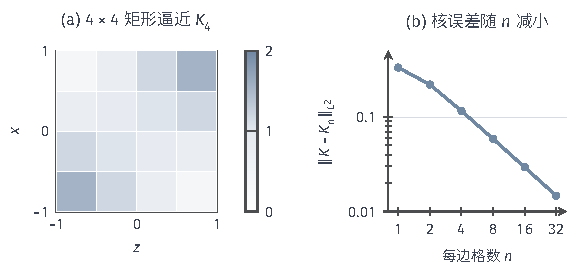
\includegraphics[width=97.4mm]{figures/02-abstract-mathematics/03-function-spaces/tikz/c3-rectangle-kernel/figure.pdf}
  \caption{用矩形示性函数的线性组合逼近核$K(x,z)=1+xz$（测度$dz/2$的乘积）。(a) $4\times4$均匀网格上取格内平均得到的分片常数核$K_4$，每格对应一个矩形$B_i\times A_j$。(b) $n\times n$网格平均的误差$\|K-K_n\|_{L^2}$，从$n=1$时的$1/3$降到$n=32$时约$0.015$，大致按$1/n$下降；它同时是相应有限秩算子的算子范数误差上界。}
  \label{fig:ose-rectangle-kernel}
\end{figure}

图~\ref{fig:ose-rectangle-kernel}在贯穿例子上演示第二步。用$n\times n$网格上的格内平均作分片常数核$K_n$，它是$n^2$个矩形示性函数的线性组合，对应的积分算子秩不超过$n$。格宽为$h=2/n$时，误差平方等于各格中$(xz-\bar x_i\bar z_j)^2$的平均，其中$\bar x_i,\bar z_j$为格中心；直接计算得$n=1,2,4,8$时误差约为$0.333$、$0.220$、$0.116$、$0.059$。对这个核，分片常数逼近远不是最经济的：$K$本身秩为$2$，截断奇异值分解两项就精确。矩形逼近的价值在于它对任意平方可积核都可行，从而在不知道奇异值的情况下证明了紧性。

\subsection{核的对称性与算子伴随}
\label{sec:ose-kernel-symmetry}

第~\ref{sec:ose-spectral-theorem}小节的谱分解要求算子自伴。本小节说明，对平方可积核，伴随算子仍是积分算子，其核由原核交换变量并取共轭得到；由此可以直接从核判断自伴性。

\paragraph{伴随核}
伴随由等式$\langle g,Tf\rangle=\langle T^*g,f\rangle$确定。左边是一个二重积分，只要能交换积分次序，就可以把对$y$的积分移到$g$一侧，读出$T^*g$的公式。

\begin{theorem}[伴随核]
\label{thm:ose-adjoint-kernel}
在定理~\ref{thm:ose-hs-bounded}的条件下，$T:L^2(\mu)\to L^2(\nu)$的伴随$T^*:L^2(\nu)\to L^2(\mu)$是以
\[
  K^*(x,y)=\overline{K(y,x)}
\]
为核的积分算子，即$(T^*g)(x)=\int_Y\overline{K(y,x)}g(y)\,d\nu(y)$。
\end{theorem}

\begin{proof}
任取$f\in L^2(\mu)$、$g\in L^2(\nu)$。函数$(y,x)\mapsto|g(y)||K(y,x)||f(x)|$在乘积空间上可积：由乘积空间中的Cauchy–Schwarz不等式，它的积分不超过$\|K\|_{L^2}$乘以$(y,x)\mapsto|g(y)f(x)|$的$L^2$范数，后者由Tonelli定理等于$\|g\|\|f\|$。于是可以用Fubini定理交换积分次序：
\[
  \begin{aligned}
  \langle g,Tf\rangle&=\int_Y\overline{g(y)}\int_XK(y,x)f(x)\,d\mu(x)\,d\nu(y)\\
  &=\int_X\overline{\Bigl(\int_Y\overline{K(y,x)}g(y)\,d\nu(y)\Bigr)}f(x)\,d\mu(x).
  \end{aligned}
\]
括号中的函数正是以$K^*$为核的积分算子作用于$g$，且$K^*\in L^2(\mu\otimes\nu)$，由定理~\ref{thm:ose-hs-bounded}它属于$L^2(\mu)$。上式说明它满足伴随的定义式$\langle g,Tf\rangle=\langle T^*g,f\rangle$；由伴随的唯一性，它就是$T^*g$。
\end{proof}

伴随核把原核的输入、输出两个变量互换，在实值情形下就是关于对角线作镜像。图~\ref{fig:ose-kernel-adjoint}以例~\ref{ex:ose-volterra-svd}中的积分算子为例：$K(x,t)=\mathbf 1_{\{t<x\}}$在对角线上方取一，表示$(Vf)(x)$累积$x$左边的输入；伴随核在对角线下方取一，表示$(V^*g)(t)=\int_t^1g$累积$t$右边的输入。这正是例中通过交换积分次序得到的公式。

\begin{figure}[!htb]
  \centering
  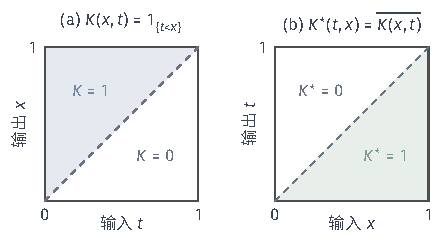
\includegraphics[width=75.2mm]{figures/02-abstract-mathematics/03-function-spaces/tikz/c3-kernel-adjoint/figure.pdf}
  \caption{积分核与伴随核关于对角线互为镜像。(a) $(Vf)(x)=\int_0^xf$的核$K(x,t)=\mathbf 1_{\{t<x\}}$，纵轴为输出变量，阴影处取值$1$。(b) 伴随核$K^*(t,x)=\overline{K(x,t)}=\mathbf 1_{\{x>t\}}$，给出$(V^*g)(t)=\int_t^1g$。两核不相等，所以$V$不自伴。}
  \label{fig:ose-kernel-adjoint}
\end{figure}

\paragraph{对称核与自伴}
当$X=Y$且$\mu=\nu$时，若$K(x,z)=\overline{K(z,x)}$对$\mu\otimes\mu$几乎处处的$(x,z)$成立，则$K^*=K$几乎处处，由定理~\ref{thm:ose-adjoint-kernel}得$T^*=T$，$T$是紧自伴算子。这时定理~\ref{thm:ose-compact-selfadjoint}的谱分解可以直接使用。实值核的这一条件就是对称性$K(x,z)=K(z,x)$。贯穿例子的$1+xz$是实对称核，所以它的特征函数$1$与$\sqrt3x$正交、特征值是实数，与第~\ref{sec:ose-spectral-theorem}小节的计算一致；积分算子$V$的核不对称，它的左右奇异函数是两组不同的三角函数。

\paragraph{对称不等于正}
自伴只说明二次型$\langle f,Tf\rangle$是实数，并不保证它非负。核$1-6xz$实对称，但取$f=x$得$Tf=-2x$，
\[
  \langle f,Tf\rangle=\int x\cdot(-2x)\,d\mu=-\tfrac23<0 .
\]
相比之下，$1+xz$给出$\langle f,Tf\rangle=|\int f\,d\mu|^2+|\int xf\,d\mu|^2\geq0$，是正算子。正性要单独检查，不能从核对称推出。

\paragraph{等价类与点值}
平方可积核本身只是$\nu\otimes\mu$几乎处处的等价类。在零测集上改动核不改变积分算子，却可能完全改变它在个别点上的取值。例如在$[-1,1]^2$上令$K'(x,z)=1+xz-10\cdot\mathbf 1_{\{x=z\}}$，对角线在乘积测度下为零测集，所以$K'$与$K$给出同一个正算子；但$K'(x,x)=x^2-9<0$，单点$\{x\}$上的$1\times1$“Gram矩阵”为负。因此，从本节的$L^2$结论出发，不能谈论“所有有限点集上的Gram矩阵是否半正定”，也不能谈论核在指定点上的再生关系。这些问题需要核取连续代表、并对所有有限点集半正定，属于第~\ref{sec:rkhs-point-evaluation}节及第~\ref{sec:rkhs-mercer}节的内容。

% 第3章第4节：积分方程的可解性与稳定性（两类方程、小范数迭代、紧算子的Fredholm二择、第一类方程与小奇异值）。

\section{积分方程的可解性与稳定性}
\label{sec:ose-integral-equations}

前三节都在正向使用算子：给定输入，计算输出。本节反过来，把积分算子放进未知函数满足的方程，依次回答章首的三个问题：解是否存在、是否唯一、对数据的误差是否稳定。两类方程的像空间结构截然不同，所以分开处理：第二类方程在小范数条件下可以直接迭代求解，在紧性条件下有完整的可解性判别；第一类方程还要面对小奇异值带来的放大。

\subsection{第一类与第二类积分方程}
\label{sec:ose-equation-types}

\paragraph{两类方程}
设$T$是积分算子，$g$是已知函数，$f$是未知函数。若$T:H_1\to H_2$，方程
\begin{equation}
  Tf=g
  \label{eq:ose-first-kind}
\end{equation}
称为\term{第一类积分方程}（integral equation of the first kind），此时$g$是观察到的输出，要求恢复产生它的输入。若$T:H\to H$，$\lambda\in\mathbb F$为参数，方程
\begin{equation}
  (I-\lambda T)f=g,\qquad\text{即}\quad f(x)-\lambda\int K(x,z)f(z)\,d\mu(z)=g(x),
  \label{eq:ose-second-kind}
\end{equation}
称为\term{第二类积分方程}（integral equation of the second kind），此时$g$是源项，未知函数同时出现在积分内外。两类方程的区别不在于写法：第二类方程中，未知函数在积分之外还有一个单位算子的“副本”，这个副本保证了在积分算子看不见的方向上，信息不会丢失。

\paragraph{贯穿例子中的两类方程}
回到$L^2([-1,1],\mu)$、$d\mu=dz/2$、$K(x,z)=1+xz$。由第~\ref{sec:ose-spectral-theorem}小节，任意$f$可以分解为$f=\alpha+\beta x+h$，其中$h$与$1,x$都正交，并且$Tf=\alpha+\frac{\beta}{3}x$。

第一类方程$Tf=g$只能产生一次函数，所以只有当$g=a+bx$时才有解。此时$\alpha=a$、$\beta=3b$，而$h$完全不受约束：
\[
  f=a+3bx+h,\qquad h\perp1,\ h\perp x .
\]
解存在时有无穷多个，差别正是$\ker T$中的任意元素，这个核是无限维的。

第二类方程$(I-\lambda T)f=g$则不同。把$g$同样分解为$g=a+bx+k$，$k$与$1,x$正交，逐方向比较系数得
\[
  (1-\lambda)\alpha=a,\qquad\Bigl(1-\frac{\lambda}{3}\Bigr)\beta=b,\qquad h=k .
\]
只要$\lambda\neq1,3$，每个$g$都给出唯一解；例如$\lambda=1/2$时$f=2a+\frac65bx+k$。图~\ref{fig:ose-equation-types}比较两类方程在各方向上的乘子：第一类方程把与$1,x$正交的方向全部乘以零，第二类方程在这些方向上保留单位作用，只在两个特征方向上改变比例。

\begin{figure}[!htb]
  \centering
  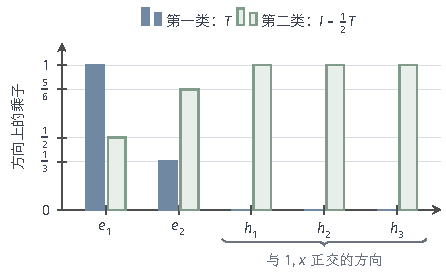
\includegraphics[width=75.5mm]{figures/02-abstract-mathematics/03-function-spaces/tikz/c3-equation-types/figure.pdf}
  \caption{核$1+xz$（测度$dz/2$）给出的两类方程在各正交方向上的乘子。$e_1=1$、$e_2=\sqrt3x$为特征方向，$h_1,h_2,h_3$代表与它们正交的方向（如$x^2-1/3$）。深色：第一类方程的算子$T$，在正交方向上为零，信息丢失；浅色：第二类方程的算子$I-\frac12T$，在正交方向上恒为$1$。}
  \label{fig:ose-equation-types}
\end{figure}

\paragraph{核、像与例外参数}
同一个例子已经显示出两类方程各自的困难。第一类方程的困难来自$T$本身：$\ker T$非零造成不唯一，$\operatorname{Ran}T$不是全空间造成不存在。第二类方程只在特殊参数处出问题：$\lambda=1$时齐次方程$(I-T)f=0$有非零解$f=1$，$\lambda=3$时有非零解$f=x$；这两个参数正是特征值$1$与$1/3$的倒数。

由此形成本节其余部分的分工。第~\ref{sec:ose-neumann}小节说明，当$\|\lambda T\|<1$时，第二类方程可以用级数和迭代直接构造解；第~\ref{sec:ose-fredholm}小节用紧性给出第二类方程对所有参数的可解性判别；第~\ref{sec:ose-first-kind}小节回到第一类方程，说明除了正交条件，还需要控制反演时被除掉的小奇异值。

\subsection{小范数条件下的解与迭代}
\label{sec:ose-neumann}

\paragraph{Neumann级数}
标量方程$(1-q)x=g$在$|q|<1$时有解$x=\sum_{n\geq0}q^ng$。算子方程可以照此办理，只要几何级数在算子范数下收敛。第~\ref{sec:lfo-operator-space}节已经证明，$X$为Banach空间时$\mathcal B(X)$在算子范数下完备，这正是让级数收敛所需要的。

\begin{theorem}[Neumann级数]
\label{thm:ose-neumann}
设$X$为Banach空间，$S\in\mathcal B(X)$且$\|S\|<1$。则$I-S$可逆，逆算子有界，并且
\[
  (I-S)^{-1}=\sum_{n=0}^{\infty}S^n,\qquad\|(I-S)^{-1}\|\leq\frac{1}{1-\|S\|},
\]
级数按算子范数收敛。
\end{theorem}

\begin{proof}
由$\|S^n\|\leq\|S\|^n$，级数$\sum_n\|S^n\|$被收敛的几何级数控制，部分和$P_N=\sum_{n=0}^{N}S^n$在$\mathcal B(X)$中是柯西列，由完备性收敛到某个$P$，且$\|P\|\leq\sum_n\|S\|^n=1/(1-\|S\|)$。部分和满足望远镜恒等式
\[
  P_N(I-S)=(I-S)P_N=I-S^{N+1},
\]
而$\|S^{N+1}\|\leq\|S\|^{N+1}\to0$。令$N\to\infty$，由算子乘法对算子范数连续，得$P(I-S)=(I-S)P=I$。
\end{proof}

由该级数定义的
\[
  \sum_{n=0}^{\infty}S^n
\]
称为\term{Neumann级数}（Neumann series）。取$S=\lambda T$，当$\|\lambda T\|<1$时，第二类方程~\eqref{eq:ose-second-kind}对每个$g$有唯一解$f=\sum_n\lambda^nT^ng$，且$\|f\|\leq\|g\|/(1-|\lambda|\|T\|)$。数据误差的影响由同一个界控制：若源项从$g$变为$\tilde g$，解的变化不超过$\|g-\tilde g\|/(1-\|\lambda T\|)$。

\paragraph{压缩迭代}
Neumann级数的部分和可以逐步计算。令$\Phi(f)=g+\lambda Tf$，则方程~\eqref{eq:ose-second-kind}等价于不动点方程$f=\Phi(f)$。从$f_0$出发迭代$f_{n+1}=\Phi(f_n)$，展开得
\[
  f_n=\sum_{k=0}^{n-1}(\lambda T)^kg+(\lambda T)^nf_0 ,
\]
即Neumann级数的部分和加上一项逐渐消失的初值影响。这个迭代满足本卷“度量空间”章压缩映射定理（定理~\ref{thm:metric-contraction}）的全部条件：$X$完备；$\Phi$把$X$映入自身；对任意$f,h$有
\[
  \|\Phi(f)-\Phi(h)\|=\|\lambda T(f-h)\|\leq q\|f-h\|,\qquad q=\|\lambda T\|<1 .
\]
压缩常数$q$对所有输入统一成立，这是压缩映射定理要求的，也是小范数条件提供的。

\paragraph{误差估计}
压缩映射定理的先验估计~\eqref{eq:metric-a-priori}直接给出
\[
  \|f_n-f_*\|\leq\frac{q^n}{1-q}\|f_1-f_0\| .
\]
若每步迭代都带有执行误差，即实际计算的$f_{n+1}$满足$\|f_{n+1}-\Phi(f_n)\|\leq\eta_n$，记$e_n=\|f_n-f_*\|$，第~\ref{sec:metric-inexact-contraction}节的递推~\eqref{eq:metric-inexact-error}给出$e_{n+1}\leq qe_n+\eta_n$。在$\eta_n\leq\eta$时，展开递推得到$\limsup_ne_n\leq\eta/(1-q)$：每步的执行误差被放大$1/(1-q)$倍，形成一个误差地板。$q$接近$1$时，即使每步误差很小，最终误差也可能很大。

\begin{example}[迭代求解第二类方程]
\label{ex:ose-neumann-iteration}
在贯穿例子中取$\lambda=1/2$，$g=1+x$。此时$q=\|\frac12T\|=\frac12$。由前一小节的系数关系，精确解为$f_*=2+\frac65x$。从$f_0=0$迭代，常数系数满足$a_{n+1}=1+\frac12a_n$，$x$的系数满足$b_{n+1}=1+\frac16b_n$，所以
\[
  a_n=2\bigl(1-2^{-n}\bigr),\qquad b_n=\tfrac65\bigl(1-6^{-n}\bigr),
\]
误差为
\[
  \|f_n-f_*\|^2=\bigl(2\cdot2^{-n}\bigr)^2+\tfrac13\bigl(\tfrac65\cdot6^{-n}\bigr)^2 .
\]
这里用到$\|\alpha+\beta x\|^2=|\alpha|^2+|\beta|^2/3$。先验界为$\frac{2^{-n}}{1/2}\|g\|=2\cdot2^{-n}\cdot\frac{2}{\sqrt3}$，比实际误差略大。若每步都多加一个$-10^{-3}$的常数偏差，常数系数改为收敛到$2-2\times10^{-3}$，误差停在$2\times10^{-3}=\eta/(1-q)$，恰好达到误差地板。
\end{example}

\begin{figure}[!htb]
  \centering
  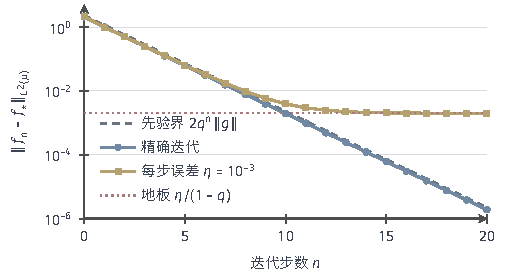
\includegraphics[width=85.7mm]{figures/02-abstract-mathematics/03-function-spaces/tikz/c3-neumann-error/figure.pdf}
  \caption{第二类方程$(I-\frac12T)f=1+x$（核$1+xz$，测度$dz/2$）的不动点迭代误差，纵轴取对数。虚线：先验界$q^n\|f_1-f_0\|/(1-q)$，$q=1/2$；圆点：精确迭代，误差几乎按$2^{-n}$下降；方点：每步带有大小$\eta=10^{-3}$的常数偏差，误差停在点线所示的地板$\eta/(1-q)=2\times10^{-3}$。}
  \label{fig:ose-neumann-error}
\end{figure}

图~\ref{fig:ose-neumann-error}画出例~\ref{ex:ose-neumann-iteration}的三条曲线。精确迭代的误差几乎贴着先验界下降，速度由最慢的方向$a_n$的比例$1/2$决定；带执行误差的迭代起初与精确迭代重合，大约十步后停在地板上，继续迭代不再改进。

\paragraph{小范数只是充分条件}
$\|\lambda T\|<1$保证可解，但不是可解的必要条件。最简单的例子是$B=2I$：$\|B\|=2$，Neumann级数$\sum_nB^n=\sum_n2^nI$发散，迭代$f_{n+1}=g+2f_n$从$f_0=0$出发给出$f_n=(2^n-1)g$，也发散；可是$I-B=-I$显然可逆，方程$(I-B)f=g$的唯一解为$f=-g$。这里的$B$不是用平方可积核表示的积分算子，只用来说明一般算子的情形。

积分方程中也有同样的现象。贯穿例子中取$\lambda=2$，则$\|\lambda T\|=2$，但$\lambda\neq1,3$，方程$(I-2T)f=g$对每个$g=a+bx+k$有唯一解$f=-a+3bx+k$。迭代的常数系数却满足$a_{n+1}=a+2a_n$，只要$a\neq0$就发散。方程可解与某个迭代法收敛是两件事；要判断前者，需要下一小节的工具。

\subsection{紧算子条件下的可解性}
\label{sec:ose-fredholm}

小范数条件把第二类方程限制在$|\lambda|<1/\|T\|$的范围内。对紧算子，我们能对所有参数给出完整的判别。先在紧自伴情形中用特征方向看清答案，再对一般紧算子给出证明。

\paragraph{紧自伴情形的方向解释}
设$T$为紧自伴算子，按定理~\ref{thm:ose-compact-selfadjoint}有特征对$(\lambda_j,e_j)$及$u=u_0+\sum_jc_je_j$，其中$u_0\in\ker T$，$c_j=\langle e_j,u\rangle$。则
\[
  (I-\lambda T)u=u_0+\sum_j(1-\lambda\lambda_j)c_je_j .
\]
$I-\lambda T$在核方向上作用为$1$，在第$j$个特征方向上乘以$1-\lambda\lambda_j$。若$\lambda$不等于任何$1/\lambda_j$，这些乘子都非零；又因为$\lambda_j\to0$，乘子趋于$1$，所以$\inf_j|1-\lambda\lambda_j|>0$。逐方向除以乘子就得到有界逆：
\[
  f=g_0+\sum_j\frac{\langle e_j,g\rangle}{1-\lambda\lambda_j}e_j ,\qquad g_0\text{为}g\text{在}\ker T\text{上的分量}.
\]
若$\lambda=1/\lambda_k$，乘子在$\lambda_k$的特征空间上为零，这个有限维特征空间就是齐次方程的解空间$\ker(I-\lambda T)$；方程可解当且仅当$g$在这些方向上的系数为零，即$g\perp\ker(I-\lambda T)$，此时解可以加上该特征空间中的任意元素。$\lambda$为实数，$I-\lambda T$自伴，所以这里的正交条件也就是$g\perp\ker(I-\lambda T)^*$。

图~\ref{fig:ose-fredholm-alternative}在贯穿例子上画出三个乘子随$\lambda$的变化。常数方向的乘子$1-\lambda$在$\lambda=1$处为零，线性方向的乘子$1-\lambda/3$在$\lambda=3$处为零，正交补方向的乘子恒为$1$。除这两个例外参数外，方程总是唯一可解的；$\lambda=1/2$与$\lambda=2$都在这个范围内，尽管只有前者满足小范数条件。

\begin{figure}[!htb]
  \centering
  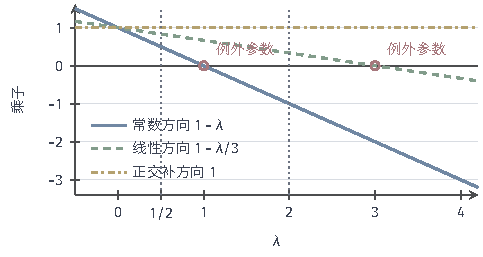
\includegraphics[width=81.8mm]{figures/02-abstract-mathematics/03-function-spaces/tikz/c3-fredholm-alternative/figure.pdf}
  \caption{第二类方程$(I-\lambda T)f=g$在各方向上的乘子随参数$\lambda$的变化（核$1+xz$，测度$dz/2$）。乘子为零的$\lambda=1$与$\lambda=3$（空心圆）是例外参数，齐次方程在此有非零解；其余参数下方程唯一可解。点线标出$\lambda=1/2$（满足小范数条件）与$\lambda=2$（不满足，但仍唯一可解）。}
  \label{fig:ose-fredholm-alternative}
\end{figure}

\paragraph{Fredholm二择定理}
对一般紧算子，没有正交特征基可用，但结论的形式保持不变。

\begin{theorem}[Fredholm二择定理]
\label{thm:ose-fredholm}
设$H$为Hilbert空间，$T:H\to H$为紧算子，$\lambda\in\mathbb F$，$B=I-\lambda T$。则：
\begin{enumerate}
  \item $\ker B$与$\ker B^*$都是有限维的；
  \item $\operatorname{Ran}B$是闭子空间，因而$\operatorname{Ran}B=(\ker B^*)^\perp$；
  \item $\ker B=\{0\}$当且仅当$\operatorname{Ran}B=H$，此时$B^{-1}$有界。
\end{enumerate}
因此以下二者恰有一个成立：齐次方程$Bf=0$只有零解，此时对每个$g\in H$，方程$Bf=g$有唯一解，且解有界地依赖于$g$；或者齐次方程有非零解，此时$Bf=g$可解当且仅当$g\perp\ker B^*$，全部解为一个特解加上$\ker B$中的任意元素。
\end{theorem}

这个结论称为\term{Fredholm二择定理}（Fredholm alternative）。它的力量在于第二条：像空间闭合是事先由紧性保证的，所以正交条件$g\perp\ker B^*$判断的是\emph{精确}可解，而不只是$g$能否被输出逼近。对比第~\ref{sec:lfo-range-kernel}节中的$A(x_n)=(x_n/n)$：$\ker A^*=\{0\}$，每个$y$都满足正交条件，但$(1/n)$并不在像中，因为$\operatorname{Ran}A$不闭。还可以证明$\dim\ker B=\dim\ker B^*$，这里不需要这一结论，不再展开。

\paragraph{证明思路：有限秩加小范数余项}
证明把紧算子拆成两部分：有限秩部分化为有限维线性方程组，余项部分用Neumann级数吸收。$\lambda=0$时$B=I$，结论显然，下面设$\lambda\neq0$。

\begin{proof}
第一步，分解。由定理~\ref{thm:ose-finite-rank-approx}，取有限秩算子$F$使$\|\lambda(T-F)\|<1$。记$C=I-\lambda(T-F)$，由定理~\ref{thm:ose-neumann}，$C$可逆且$C,C^{-1}$都有界。于是
\[
  B=C-\lambda F=C(I-G),\qquad G=\lambda C^{-1}F .
\]
$G$仍是有限秩算子。取$\operatorname{Ran}G$的一组线性无关基$b_1,\ldots,b_r$，则$Gf=\sum_{i=1}^r\ell_i(f)b_i$，系数$\ell_i$是有界线性泛函，由Riesz表示（第~\ref{sec:lfo-riesz}节）写成$\ell_i(f)=\langle a_i,f\rangle$。

第二步，化为矩阵方程。令$\bm M_{i,j}=\langle a_i,b_j\rangle$，$\bm d(h)=(\langle a_1,h\rangle,\ldots,\langle a_r,h\rangle)^\top$。我们断言：$(I-G)f=h$当且仅当$f=h+\sum_ic_ib_i$，其中$\bm c=(c_1,\ldots,c_r)^\top$满足$(\bm I-\bm M)\bm c=\bm d(h)$。若$(I-G)f=h$，则$f=h+Gf=h+\sum_ic_ib_i$，其中$c_i=\langle a_i,f\rangle=\langle a_i,h\rangle+\sum_j\bm M_{i,j}c_j$。反过来，若$\bm c$满足矩阵方程，令$f=h+\sum_jc_jb_j$，则$Gf=\sum_i\bigl(\bm d(h)_i+(\bm M\bm c)_i\bigr)b_i=\sum_ic_ib_i=f-h$。

第三步，核有限维、像闭合。取$h=0$，$\ker(I-G)$由$\ker(\bm I-\bm M)$经单射$\bm c\mapsto\sum_ic_ib_i$得到，维数不超过$r$；$C$可逆，所以$\ker B=\ker(I-G)$有限维。由第二步，$h\in\operatorname{Ran}(I-G)$当且仅当$\bm d(h)\in\operatorname{Ran}(\bm I-\bm M)$。$\mathbb F^r$的子空间$\operatorname{Ran}(\bm I-\bm M)$是有限个线性泛函的公共零点，与连续映射$\bm d$复合后，$\operatorname{Ran}(I-G)$是$H$上有限个连续线性泛函的公共零点，因而闭。$C$与$C^{-1}$都连续，所以$\operatorname{Ran}B=C\bigl(\operatorname{Ran}(I-G)\bigr)$也闭。

第四步，单射推出满射。若$\ker B=\{0\}$，则$\ker(\bm I-\bm M)=\{0\}$，有限维方阵$\bm I-\bm M$可逆，矩阵方程对每个$\bm d(h)$有解，于是$I-G$满射，$B=C(I-G)$也满射。反之，若$B$满射，则$\ker B^*=(\operatorname{Ran}B)^\perp=\{0\}$；对下一步说明的紧算子$T^*$应用本步，$B^*$满射，从而$\ker B=(\operatorname{Ran}B^*)^\perp=\{0\}$。双射$B$的逆有界由第~\ref{sec:lfo-open-mapping}节的有界逆定理保证。

第五步，处理伴随。若$F_n$是有限秩算子且$\|T-F_n\|\to0$，则$F_n^*$也是有限秩的（$F_nf=\sum_i\langle a_i,f\rangle b_i$时$F_n^*g=\sum_i\langle b_i,g\rangle a_i$），且$\|T^*-F_n^*\|=\|T-F_n\|\to0$，由定理~\ref{thm:ose-compact-limit}，$T^*$是紧算子。$B^*=I-\overline\lambda T^*$与$B$同型，由第三步，$\ker B^*$有限维。最后，像闭合且由第~\ref{sec:lfo-range-kernel}节$\overline{\operatorname{Ran}B}=(\ker B^*)^\perp$，得$\operatorname{Ran}B=(\ker B^*)^\perp$。
\end{proof}

第三步中，有限维的矩阵方程决定了无限维方程的全部可解性：无限维部分已经被可逆的$C$吸收。这也说明了紧性的作用：若$T$不能被有限秩算子逼近，就无法把问题化到有限维。

\paragraph{两个推论}
定理的第三条有一个直接推论：紧算子$T$的非零谱点都是特征值。若$\mu\neq0$不是特征值，取$\lambda=1/\mu$，则$I-\lambda T$是单射，由定理是有界可逆的，于是$T-\mu I=-\mu(I-\lambda T)$也有界可逆，$\mu\in\rho(T)$。结合第~\ref{sec:ose-spectrum-def}小节，无限维空间中紧算子的谱由至多可数个非零特征值和$0$组成。

另一个推论关于迭代。Fredholm二择告诉我们方程何时可解，但没有给出求解的迭代格式。第~\ref{sec:ose-neumann}小节中$\lambda=2$的例子正处于“唯一可解但迭代发散”的情形：定理~\ref{thm:ose-fredholm}保证解存在、有界依赖于数据，固定点迭代仍受$\|\lambda T\|<1$的收缩条件限制。

\subsection{第一类方程与小奇异值}
\label{sec:ose-first-kind}

第一类方程$Tf=g$没有单位算子的“副本”，紧算子$T$的像一般不闭，Fredholm二择的结论不再适用。本小节用奇异值分解给出精确可解的条件，并说明为什么即使解存在，它也可能对数据极其敏感。

\paragraph{精确可解的Picard条件}
设$T:H_1\to H_2$为紧算子，奇异值分解为$Tx=\sum_j\sigma_j\langle v_j,x\rangle u_j$。若$Tf=g$，则对每个$j$，
\[
  \langle u_j,g\rangle=\langle u_j,Tf\rangle=\langle T^*u_j,f\rangle=\sigma_j\langle v_j,f\rangle ,
\]
所以$f$在$v_j$方向上的系数只能是$\langle u_j,g\rangle/\sigma_j$。这些系数必须平方可和，$f$才属于$H_1$。

\begin{theorem}[第一类方程的可解性与最小范数解]
\label{thm:ose-picard}
设$T:H_1\to H_2$为紧算子，奇异值分解如定理~\ref{thm:ose-svd}。则$Tf=g$有解，当且仅当以下两条同时成立：
\begin{equation}
  g\perp\ker T^*,\qquad \sum_j\frac{|\langle u_j,g\rangle|^2}{\sigma_j^2}<\infty .
  \label{eq:ose-picard}
\end{equation}
此时
\[
  f^\dagger=\sum_j\frac{\langle u_j,g\rangle}{\sigma_j}v_j
\]
是唯一属于$(\ker T)^\perp$的解，全部解为$f^\dagger+\ker T$，且$f^\dagger$是范数最小的解。
\end{theorem}

\begin{proof}
必要性：若$Tf=g$，则$g\in\operatorname{Ran}T\subseteq(\ker T^*)^\perp$；由上面的系数关系和Bessel不等式，$\sum_j|\langle u_j,g\rangle|^2/\sigma_j^2=\sum_j|\langle v_j,f\rangle|^2\leq\|f\|^2$。

充分性：第二个条件使级数$f^\dagger$按范数收敛（第~\ref{sec:fs-orthogonal-expansion}节），且$f^\dagger$属于$(v_j)$的闭张成$(\ker T)^\perp$。由连续性逐项作用，$Tf^\dagger=\sum_j\langle u_j,g\rangle u_j$，这是$g$在$(u_j)$的闭张成上的正交投影。由定理~\ref{thm:ose-svd}，这个闭张成等于$(\ker T^*)^\perp$，而第一个条件说明$g$就在其中，所以$Tf^\dagger=g$。

解的结构：两个解之差属于$\ker T$，故全部解为$f^\dagger+\ker T$。$(\ker T)^\perp$中的解唯一，因为两个这样的解之差同时属于$\ker T$与$(\ker T)^\perp$。对任意解$f=f^\dagger+h$，$h\in\ker T$与$f^\dagger$正交，由勾股定理$\|f\|^2=\|f^\dagger\|^2+\|h\|^2\geq\|f^\dagger\|^2$。
\end{proof}

式~\eqref{eq:ose-picard}中的第二个条件称为\term{Picard条件}（Picard condition），$f^\dagger$称为\term{最小范数解}（minimum-norm solution）。两个条件分工不同：第一个只保证$g$位于像的闭包中，即$g$能被输出任意逼近；第二个才保证形式逆像$\sum_j\sigma_j^{-1}\langle u_j,g\rangle v_j$真正属于输入空间。

\paragraph{Picard条件的例子}
在贯穿例子中，$T$只有两个奇异值$1$与$1/3$，Picard条件自动成立，第一个条件就是$g\in\operatorname{span}\{1,x\}$；对$g=a+bx$，最小范数解为$f^\dagger=a+3bx$，与第~\ref{sec:ose-equation-types}小节的结果一致，它正是全部解中去掉核分量$h$的那一个。

$\ell^2$上的$A(x_n)=(x_n/n)$说明两个条件确实不同。$A$自伴且单射，$\ker A^*=\{0\}$，第一个条件对所有$g$成立；奇异值$\sigma_n=1/n$，Picard条件化为$\sum_nn^2|g_n|^2<\infty$。图~\ref{fig:ose-picard-coefficients}比较两组数据：$g^{(1)}_n=1/n^2$的形式解系数为$1/n$，平方可和，$g^{(1)}=A(1/n)$；$g^{(2)}_n=1/n$本身平方可和，但形式解系数恒为$1$，不平方可和，所以$g^{(2)}$不在像中。这正是第~\ref{sec:lfo-range-kernel}节的例子，现在由Picard条件统一解释。

\begin{figure}[!htb]
  \centering
  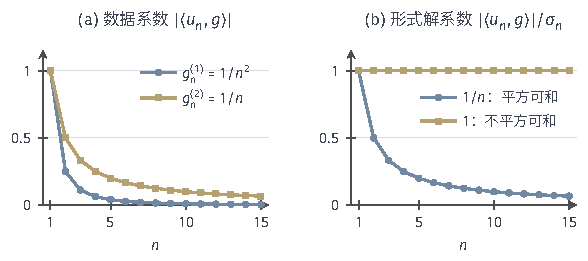
\includegraphics[width=99.6mm]{figures/02-abstract-mathematics/03-function-spaces/tikz/c3-picard-coefficients/figure.pdf}
  \caption{$\ell^2$上$A(x_n)=(x_n/n)$的Picard条件。(a) 两组数据的系数$1/n^2$与$1/n$，都平方可和，都满足$g\perp\ker A^*$。(b) 除以奇异值$\sigma_n=1/n$后的形式解系数：前者为$1/n$，平方可和，方程可解；后者恒为$1$，不平方可和，方程无解。}
  \label{fig:ose-picard-coefficients}
\end{figure}

对例~\ref{ex:ose-volterra-svd}的积分算子$V$，若$g$绝对连续、$g(0)=0$且$g'\in L^2(0,1)$，分部积分并利用$\cos\omega_k=0$可得$\langle u_k,g\rangle=\sigma_k\langle v_k,g'\rangle$，于是Picard级数等于$\sum_k|\langle v_k,g'\rangle|^2=\|g'\|^2$，最小范数解就是$f^\dagger=g'$。求解第一类方程$Vf=g$就是求导，这与微分运算的不稳定性一致。

\paragraph{小奇异值放大扰动}
即使解存在，它对数据的依赖也可能没有统一的界。设$T$有无限多个正奇异值，$\sigma_j\to0$。取数据扰动$\delta g_j=\sigma_ju_j$，则$\|\delta g_j\|=\sigma_j\to0$；它满足Picard条件，相应的最小范数解扰动为
\[
  \delta f_j=\frac{\langle u_j,\delta g_j\rangle}{\sigma_j}v_j=v_j,\qquad\|\delta f_j\|=1 .
\]
数据误差趋于零，解的误差却始终为$1$。所以映射$g\mapsto f^\dagger$在$\operatorname{Ran}T$上无界；这也说明$\operatorname{Ran}T$不闭，否则$T$限制在$(\ker T)^\perp$上是到闭像的有界双射，由有界逆定理其逆有界。只有有限多个正奇异值时情况相反：$\|f^\dagger\|\leq\|g\|/\sigma_{\min}$，在贯穿例子中放大倍数至多为$3$。

\begin{figure}[!htb]
  \centering
  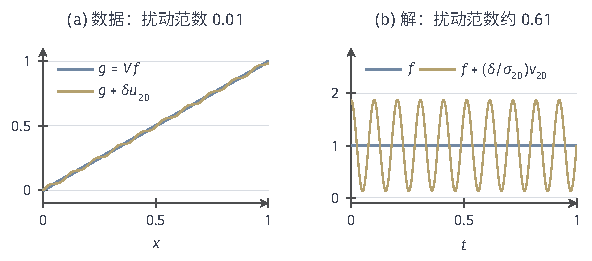
\includegraphics[width=100.2mm]{figures/02-abstract-mathematics/03-function-spaces/tikz/c3-noise-amplification/figure.pdf}
  \caption{第一类方程$Vf=g$（$(Vf)(x)=\int_0^xf$）中小奇异值放大扰动。真解$f=1$，数据$g=x$。(a) 数据加上范数为$0.01$的扰动$\delta u_{20}$，与原数据几乎重合。(b) 相应的最小范数解多出$(\delta/\sigma_{20})v_{20}$，振幅约$0.87$、范数约$0.61$，放大倍数$1/\sigma_{20}=19.5\pi\approx61$。}
  \label{fig:ose-noise-amplification}
\end{figure}

图~\ref{fig:ose-noise-amplification}在积分算子$V$上展示这一机制。数据中加入$\delta u_{20}$，$\delta=0.01$，曲线上几乎看不出差别；解中却多出振幅接近$0.87$的快速振荡。原因正是图~\ref{fig:ose-svd-decay}中看到的：$V$把快速振荡的输入平均掉，反解时必须把同样的振荡放大回去，振荡越快，放大倍数$1/\sigma_k=(k-\frac12)\pi$越大。

因此，第一类方程的解是否稳定，取决于数据在小奇异值方向上的成分。实际数据总带有误差，误差在所有方向上都有成分，直接计算$f^\dagger$会把高阶方向上的误差放大到失去意义。处理办法是舍去或压低小奇异值方向，例如只保留前$m$个奇异方向，或在求解目标中加入惩罚项；这些方法如何选择截断位置或惩罚强度、怎样平衡偏差与误差放大，属于优化问题，可参考\BookChapterRef{chap:optimization}{卷三“优化问题的定义与基本性质”章}及其后各章。从带噪观测中重建信号的具体任务，可参考\BookChapterRef{chap:signal-analysis}{卷三“信号”章}。

% 第3章第5节：本章小结。

\section{本章小结}
\label{sec:ose-summary}

章首的积分变换$Tf=\int(1+xz)f\,d\mu$只记住输入的两个矩，$\ell^2$上的$A(x_n)=(x_n/n)$则不丢掉任何方向，只是越往后压得越狠。本章围绕这两个例子，从三个角度描述一个变换：它能否用有限个方向统一逼近，各个方向被保留或压缩多少，以及从输出能否稳定地恢复输入。

紧性回答第一个问题。紧算子把有界输入族压成可以抽出收敛子列的输出族，并把弱收敛的输入变成范数收敛的输出。紧算子的算子范数极限仍是紧算子；在Hilbert空间中，紧算子恰好是有限秩算子的算子范数极限。这里的关键是“统一”：每个函数都能被截断逼近，并不意味着同一个有限维空间能以给定精度覆盖整个单位球的像，单位算子就是反例。

谱与奇异值回答第二个问题。无限维中谱不只由特征值组成，$A$的谱点$0$不对应任何被消去的方向，而对应一列越来越扁的方向和不闭的像。紧自伴算子有至多可数个实的非零特征值，只能在零处聚集，特征方向与核一起张满整个空间；一般紧算子用输入、输出两组方向写成奇异值分解，截断前$m$项的误差恰为$\sigma_{m+1}$，且是所有秩不超过$m$的逼近中最小的。这些展开都按Hilbert空间的范数成立，不自动给出逐点收敛。

积分核把上述结论具体化。核与测度一起确定算子；平方可积核给出有界的紧算子，证明的桥梁是用矩形示性函数的有限和逼近核；交换变量并取共轭得到伴随核，对称核给出自伴算子。但对称不保证正性，平方可积核作为等价类也谈不上点值和有限点集上的Gram矩阵。

第三个问题在两类方程上有不同的答案。第二类方程$(I-\lambda T)f=g$保留了单位算子，小范数时Neumann级数和压缩迭代直接给出解与误差界；对紧算子，Fredholm二择保证像闭合，于是要么唯一可解且稳定，要么在正交相容条件下可解、解差一个有限维核。第一类方程$Tf=g$还要满足Picard条件，而小奇异值使最小范数解对数据误差无界地敏感。几种判断不能互相替代：正交条件只在像闭合时判断精确可解，可解不等于某个迭代收敛，有解也不等于稳定。

这些认识是后续几类问题的起点。第~\ref{chap:rkhs}章给积分核加上连续性与半正定性，研究点值读取连续的函数空间，并在那里建立Mercer展开的逐点与一致收敛；带噪数据下怎样舍去或压低小奇异值方向，是优化中正则化的问题，具体的微分方程演化与信号重建则分别属于卷三的动力系统与信号部分。本章只保留算子方向与积分方程的共同基础，不预先引入这些任务各自的目标和算法。

